\documentclass[12pt, reqno]{report}

\usepackage{amssymb, amsmath, mathrsfs}
\usepackage{amsthm}
\usepackage[margin=2 cm]{geometry}
\usepackage{graphbox}
\usepackage{color}
\usepackage{float}
\usepackage{subfigure}
\usepackage{wrapfig}
\usepackage{array}
\usepackage{multicol}
\usepackage{caption}
\usepackage{titlesec}
\titleformat{\chapter}{}{}{0em}{\bf\LARGE}
\titlespacing*{\chapter}{0pt}{0pt}{20pt}
\usepackage[backend=bibtex, style=numeric]{biblatex}
\addbibresource{bibliography.bib}
\newtheorem{theorem}{Theorem}[section]
\newtheorem*{theorem*}{Theorem}          %theorem without number
\newtheorem{prop}{Proposition}[section]
\newtheorem*{prop*}{Proposition}  % proposition without number
\newtheorem{coro}{Corollary}[section]
\newtheorem{lemma}[theorem]{Lemma}
\newtheorem{conj}{Conjecture}[section]
\newtheorem{obs}{Observation}[section]

\theoremstyle{definition}
\newtheorem{definition}[theorem]{Definition}
\newtheorem{example}[theorem]{Example}
\newtheorem{xca}[theorem]{Exercise}

\theoremstyle{remark}
\newtheorem{remark}[theorem]{Remark}

\newcommand{\abs}[1]{\lvert#1\rvert}
\newcommand{\norm}[1]{\lVert#1\rVert}
\DeclareMathOperator{\re}{Re}
\DeclareMathOperator{\im}{Im}
\newcommand{\ud}{\mathrm{d}}
\newcommand{\e}{\mathrm{e}}
\renewcommand{\i}{\mathrm{i}}

% REMOVE DRAFT

\begin{document}

\title{Comparison of Continuum and Atomistic Models for Chemical Diffusion and Phase Separation}
\date{\today}
\author{Isaac Viviano}

\maketitle

\begin{abstract}

    We model the physical phenomena of diffusion and phase separation. Differential equations provide a continuum approximation of these processes. The heat equation models diffusion of a spatial concentration gradient. The Allen-Cahn and Cahn-Hilliard equations model phase separation of a binary mixture into its components. Each differential equation is approximated using the finite difference method. For particle-based models, the software LAMMPS is used to simulate molecular dynamics. The diffusive system studied was Argon diffusing in Helium gas. For phase separation, a two-component Leonard-Jones fluid was modeled. The qualitative behavior of the time evolution of the models is compared. Additionally, the differential equation parameters are estimated from molecular dynamics data to quantitatively connect the timescales.

\end{abstract}

\tableofcontents

\chapter{Introduction} \label{sec_intro}

This project was motivated by the influence of electrolytes on the phase separation of polymer solutions. 
We choose to take a mathematical modeling approach to similar chemical phenomena.
One fundamental question in modeling is when a course grained approximation is appropriate.
With some course grained approximations, there is the additional consideration of how to interpret results physically.
We use numerical techniques to compare an atomistic and continuum model of chemical diffusion and phase separation.
Based on the comparison, we propose a parameter estimation procedure to interpret the continuum results.
Our atomistic model uses Molecular Dynamics (MD). 
MD simulates the time evolution of a collection of classical particles.
A specific model is chosen for approximating the interparticle forces. 
Then, various dynamics can be used for the according evolution.
We conduct equilibrium MD simulations, where the particles follow Hamiltonian dynamics of pairwise Leonard-Jones interactions.
MD simulations were conducted with the open-source software LAMMPS \cite{LAMMPS}.
Our continuum models are differential equations.
Each differential equation has a physical derivation from continuum mechanical laws.
We discuss their mathematical derivations as gradient flows of energy functionals.
We present numerical algorithms based on the finite difference method to approximate solutions to each differential equation.

In the physical reality, all dynamics are quantum, and the classical approximation of MD is itself a coarse graining.
MD makes additional approximations through numerical algorithms and specific model-simplifying assumptions.
Still, for our analysis, we use MD simulations as the physical reference for evaluating the continuum course graining.
While it would be interesting to examine the advantages and disadvantages of a more accurate atomistic model, that is outside the scope of this project.
We suggest procedures to set the continuum timescale and phenomenological parameters from the MD trajectories.
Using this algorithm, we estimate the the differential equation parameters from the MD simulations, and evaluate the fitted continuum model's performance.
We model the simplest relevant physical systems, with the goal of demonstrating the estimation technique and making the continuum model feasible.

One of the strengths of MD is its ability to reveal the effect of manipulating state variables.
Estimating the differential equation parameters at different system states could determine their temperature, pressure, or concentration dependence. 
Each model may be applied to 1,2, and 3 dimensional systems.
Throughout this paper, we will denote the system dimension by $d$, when it is relevant to a derivation or result.
We present numerical results primarily in 1 and 2 dimensions. 
While the models are equally valid for $d=3$, we choose lower dimensions to reduce computational complexity and help with data visualization.
We begin by analyzing atomistic and continuum models for diffusion before moving on to phase separation.
Diffusion is an critical part of phase separation dynamics and can be accurately described by a simpler model. 

\chapter{Diffusion} \label{chap_intro}

For a system of particles under a non-zero concentration gradient, random motion tends to reduce the concentration gradient over time.
This net movement of particles from regions of higher concentration to lower concentration is called diffusion.
For real substances, the dynamics of diffusion are impacted by many factors. 
Generally, diffusion is faster at higher temperatures and lower pressures.
Fick's laws relate diffusion flux to the concentration gradient via the mass diffusivity, or diffusion coefficient.
Fick's second law will be the basis for our continuum model of diffusion.

\section{Heat Equation} \label{sec_heat}

When modeling diffusion as a continuum phenomenon, we follow the concentration of solute.
This is the order parameter of the system, and is denoted $u(x,t)$.
One continuum diffusion model comes from the heat equation.
The heat equation with periodic boundary conditions is
\begin{equation} \label{eq_HE}
    \left\{
        \begin{split}
            &\frac{\partial u}{\partial t}=D\nabla^2u&x\in\Omega,t>0\\
            &u\big|_{x_i=0}=u\big|_{x_i=1}&1\le i\le d\\
            &u_{x_i}\big|_{x_i=0}=u_{x_i}\big|_{x_i=1}&1\le i\le d\\
            &u(x,0)=u_0(x)&x\in\Omega,
        \end{split}	
    \right.
\end{equation}
where $D>0$ is the diffusion coefficient, $\Omega=[0,1]^d$ is the spatial domain, and $u_0(x)$ is the initial condition. 
For solutions $u$ to the heat equation, the concentration gradient must decrease in time, since
\begin{equation}
    \nabla^2u=\nabla\cdot\nabla u.
\end{equation}


\subsection{Analytical Solution} \label{sssec_analytical}

For the unit cube in $d$ dimensions and periodic boundary conditions, the heat equation (\ref{eq_HE}) may be solved analytically.
The solution $u$ can be written as the Fourier series
\begin{equation} \label{eq_heat_solution}
    u(x,t)=\sum_{m\in\mathbb{Z }^d}C_m ~\e^{-4\pi^2|m|^2Dt}~\mathrm{e}^{2\pi\i m\cdot x},
\end{equation}
where 
\begin{equation}
    C_m=\int_{\Omega}u_0(x)~\e^{2\pi\i m\cdot x}~\ud x 
\end{equation}
is the $m$-th Fourier coefficient of the initial condition.

From the analytical solution (\ref{eq_heat_solution}), we see that solutions $u$ to the heat equation satisfy the mass conservation constraint
\begin{equation} \label{eq_mass_con}
    \frac{\ud}{\ud t}\int_\Omega u(x,t)~\ud x=\frac{\ud}{\ud t}~C_0=0.
\end{equation}
All non-constant modes decay exponentially in time, causing $u$ to converge to its uniform average concentration as $t\to\infty$. 

\subsection{Finite Difference Approaches} \label{sssec_heat_fd}


For a numerical approximation of the differential equation, both temporal and spatial domains must be discretized. 
We choose a finite timestep $k>0$ and approximate the solution at times $t=0,k,2k,\ldots$. 
We partition each spatial coordinate into $N$ even pieces. The solution $u$ to the differential equation is then approximated by the sequence of samples
\begin{equation} \label{eq_seq_approx}
	u_j^n\approx u(jh,nk)\quad j\in[N]^d,\quad n=0,1,\ldots
\end{equation}
where the spatial resolution $h=\frac{1}{N}$ reflects the domain size and sampling rate. 
In (\ref{eq_seq_approx}) we have used the notation
\begin{equation}
    [N]:=\{0,\ldots,N-1\}.
\end{equation}

To construct the difference equation corresponding to (\ref{eq_HE}), we must also discretize the the differential operator. 
The discrete Laplacian is defined by
\begin{equation}
    \Delta^hu_j^n=\frac{1}{h^2}\sum_{i=1}^d u_{j+e_i}^n-2u_j^n+u_{j-e_i}^n,
\end{equation}
where $e_1,\ldots,e_d$ are the standard basis for $\mathbb{R}^d$.
Accordingly, we define two difference schemes for the heat equation. 
Scheme (\ref{ds_HE_FD}) 
\begin{equation} \label{ds_HE_FD}
	\frac{u_j^{n+1}-u_j^n}{k}=D\Delta^hu_j^n{\tag{S1}}.
\end{equation}
is forward Euler in time and central in space.
Scheme (\ref{ds_HE_CN})
\begin{equation} \label{ds_HE_CN}
	\frac{u_j^{n+1}-u_j^n}{k}=\frac{D}{2}(\Delta^hu_j^{n+1}+\Delta^hu_j^n){\tag{S2}}
\end{equation}
is trapezoidal in time and central in space:

Since $u_{j}^{n}$ approximates the 1-periodic function $u$, it may be interpreted as samples of a 1-periodic signal. 
This justifies writing 
\begin{equation} \label{eq_as_DFT}
    u_{j}^{n}=\sum_{m\in[N]^{d}}\alpha_{m}^{n}~\e^{2\pi\i \frac{m\cdot j}{N}},
\end{equation}
where 
\begin{equation} 
    \alpha_{m}^{n}=\sum_{j\in[N]^{d}}u_{j}^{n}~\e^{-2\pi\i \frac{m\cdot j}{N}}
\end{equation}
is the discrete Fourier transform (DFT) of the sequence $u_{j}^{n}$. 
For the $d$-dimensional DFT, the wavenumbers are vectors $m\in [N]^{d}$.

Using properties of the exponential function, we can understand how the discrete Laplacian operator acts on Fourier space.
\begin{align*}
		\Delta^{h}u_{j}^{n}&=\frac{1}{h^2}\sum_{i=1}^{d} \sum_{m\in[N]^{d}}\alpha_{m}^{n}~\left(\e^{2\pi \i \frac{m\cdot(j + e_{i})}{N}}-2\e^{2\pi\i\frac{m\cdot j}{N}}+\e^{2\pi\i\frac{m\cdot(j-e_{i})}{N}}\right)\\
		&=\sum_{m\in[N]^{d}}\sum_{i=1}^{d}\alpha_m^n\frac{1}{h^2}\left( \e^{2\pi\i\frac{m}{N}}+\e^{-2\pi\i\frac{m}{N}}-2 \right)~\e^{2\pi\i\frac{m\cdot j}{N}}\\
		&= \sum_{m\in[N]^{d}}\alpha_{m}^{n}~\e^{2\pi\i \frac{m\cdot j}{N}}\underbrace{\sum_{i=1}^{d}\e^{2\pi\i \frac{m}{N}}+\e^{-2\pi\i \frac{m}{N}}-2}_{:=\lambda_{m}} \\
		&=\sum_{m\in[N]^{d}}\lambda_m\alpha_m^n~\e^{2\pi\i\frac{m\cdot j}{N}}\\
\end{align*}
Thus, differentiation in the spatial domain corresponds to multiplication in the Fourier domain. For second-order differentiation, we have multiplication by the factor
\begin{equation}
    \lambda_{m}= \frac{1}{h^{2}}\sum_{i=1}^{d}\left(2\cos\left(2\pi \frac{m_{i}}{N}\right)-2\right)=- \frac{4}{h^{2}}\sum_{i=1}^{d}\sin^{2}\left(\pi \frac{m_{i}}{N}\right).
\end{equation}

Stability of the difference equation is defined by the DFT representation (\ref{eq_as_DFT}) of $u_{j}^{n}$. We say the algorithm is stable if 
\begin{equation} \label{eq_stab_cond}
|\alpha_{m}^{n+1}|\le |\alpha_{m}^{n}|\quad \text{for all }m.
\end{equation}
For the heat equation forward difference scheme (\ref{ds_HE_FD}), we have the equivalent equation
\begin{equation} \label{ds_HE_FD_FT}
    \alpha_{m}^{n+1}=\alpha_{m}^{n}+k D\lambda_{m}\alpha_{m}^{n}=(1+k \lambda_{m})\alpha_{m}^{n}
\end{equation} 
in Fourier space.
The quantity $1+kD\lambda_m$ is called the amplification factor of the difference scheme. 
From the amplification factor, the stability condition (\ref{eq_stab_cond}) becomes 
\begin{equation}
    |1+k D\lambda_{m}|\le1\quad \text{for all }m.
\end{equation}
Since $\lambda_{m}\le 0$, this is equivalent to 
\begin{equation}
    1+k D\lambda_{m}\ge-1.
\end{equation}
We need the minimum value of $k D\lambda_{m}$ greater than or equal to 2. 
Over all $N$ and all $m_{i}\in[N]$, the maximum of $\sin^{2} \left(\pi \frac{m_i}{N}\right)$ is 1. 
Therefore, a necessary and sufficient condition for stability is that 
\begin{equation}
    k\le \min\left\{\frac{2}{\frac{4D}{h^{2}}\sum_{i=1}^{d}\sin^{2}\left(\pi \frac{m_{i}}{N}\right)}:N\in \mathbb{N},m\in[N]^{d}\right\}= \frac{h^{2}}{2D\sum_{i=1}^{d}1}.
\end{equation}
The maximum $k$ value for which the scheme is stable is written 
\begin{equation} %\label{eq_}
k_\text{crit}:= \frac{h^{2}}{2dD}.
\end{equation}
The amplification factor is plotted in Figure \ref{fg_HE_amp} for different values of $k$, showing stability for $k\le k_\text{crit}$.

\begin{figure}[H]
    \centering

    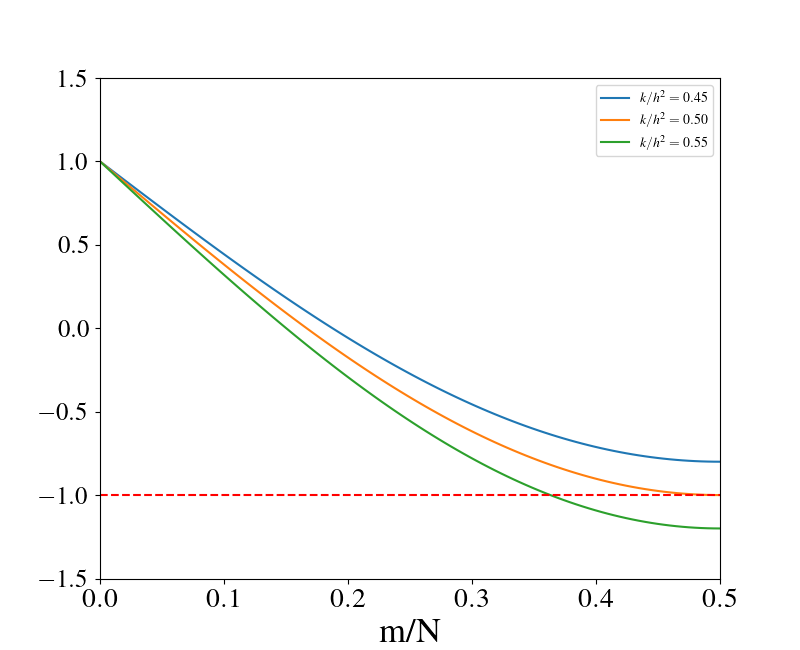
\includegraphics[width = .5\paperwidth]{media_paper/amp_HE_FD.png}

    \caption{The amplification factor for the one-dimensional heat equation forward difference scheme (\ref{ds_HE_FD}) is plotted for different values of $\frac{k}{h^2}$ near $\frac{k_\text{crit}}{h^2}$. When $k$ is above the critical value, the amplification factor dips below -1, showing a high frequency instability for the difference scheme. For simplicity, $D=1$.}
    \label{fg_HE_amp}
\end{figure}

For the implicit scheme (\ref{ds_HE_CN}), we have the equivalent equation
\begin{equation} 
    \alpha_{m}^{n+1}=\alpha_{m}^{n}+ \frac{kD}{2}(\lambda_{m}\alpha_{m}^{n+1}+\lambda_{m}\alpha_{m}^{n})
\end{equation}
in Fourier space.
Simplification gives
\begin{equation} \label{ds_HE_CN_FT}
    (1- \frac{k}{2}\lambda_{m})\alpha_{m}^{n+1}=(1+ \frac{kD}{2}\lambda_{m})\alpha_{m}^{n}\implies \frac{\alpha_{m}^{n+1}}{\alpha_{m}^{n}}= \frac{1+\frac{k}{2}\lambda_{m}}{1- \frac{kD}{2}\lambda_{m}}.
\end{equation}
Since $\lambda_{m}\le0$, this shows unconditional stability for $k>0$.
\begin{equation}
    -1\le \frac{\alpha_{m}^{n+1}}{\alpha_{m}^{n}}\le1\implies |\alpha_{m}^{n+1}|\le|\alpha_{m}^{n}|
\end{equation}


Note that each difference scheme also satisfies mass conservation. Using the Fourier space equation (\ref{ds_HE_FD_FT}), we have
\begin{equation*}
	\alpha_0^{n+1}=\alpha_0^n+kD\underbrace{\lambda_0}_{=0}\alpha_0^n=\alpha_0^n,
\end{equation*}
so
\begin{equation} \label{eq_discrete_con}
	h^2\sum_{j\in[N]^d}u_j^{n+1}=\alpha_0^{n+1}=\alpha_0^{n}=h^2\sum_{j\in[N]^d}u_j^n.
\end{equation}
Similarly for scheme (\ref{ds_HE_CN}), 
\begin{equation*}
	\alpha_0^{n+1}=\alpha_0^n+\frac{kD}{2}(\lambda_0\alpha_0^{n+1}+\lambda_0\alpha_0^n)=\alpha_0^n.
\end{equation*}

\begin{remark}
    The form of Scheme (\ref{ds_HE_CN}) given in its definition suggests an iterative process that involves solving a linear system of $N^d$ equations at each timestep.
    However, we can drastically improve complexity with the fast Fourier transform algorithm (FFT). 
    The form of Scheme (\ref{ds_HE_CN}) in (\ref{ds_HE_CN_FT}) show that in Fourier space, the iterative process can be performed in $O(n^d)$ with a single multiplication on each amplitude. 
    Therefore, using the FFT to convert back to the spatial domain results in $O(n^d\log n )$ at each timestep \cite{copetti_1990_kinetics}.
    The FFT approach was used in the implementations of all (semi)-implicit schemes.
\end{remark}

\section{Diffusion Molecular Dynamics} \label{ssec_diff_MD}

\begin{wrapfigure}{r}{.4\paperwidth}

    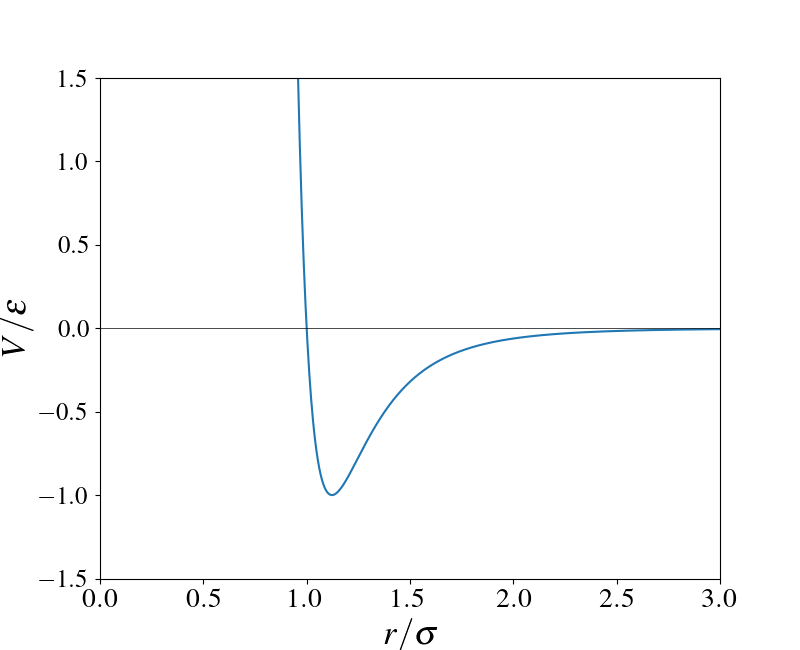
\includegraphics[width = .4\paperwidth]{media_paper/gen_lj.png}
    
    \caption{The dimensionless 6-12 Leonard-Jones potential energy function $\frac{V}{\epsilon}$ is plotted against dimensionless interparticle radius $\frac{r}{\sigma}$. The parameter $\sigma$ sets the $x$-intercept and $\epsilon$ is the maximum depth of the potential well.}
    \label{fg_lj_pot}
\end{wrapfigure}
We use the Leonard-Jones model for interparticle interactions. 
Two Leonard-Jones particles $i,j$ have the interaction potential
\begin{equation} \label{eq_6-12_pot}
    V_{ij}=
    \begin{cases}
        4\epsilon_{ij}\left[ \left( \frac{\sigma_{ij}}{r_{ij}} \right)^{12}-\left( \frac{\sigma_{ij}}{r_{ij}} \right)^6 \right]&r_{ij}<r_c\\
        0&r_{ij}\ge r_c,
    \end{cases}
\end{equation}
where $r_{ij}$ is the distance between $i$ and $j$, $\sigma_{ij}$ and $\epsilon_{ij}$ are the Leonard-Jones parameters, and $r_c$ is a range cutoff. 
The strength of interactions is determined by $\epsilon_{ij}$, which is the maximum depth of the potential well.
The distance scale of interactions is $\sigma_{ij}$, which is the distance where $V_{ij}=0$. 
Typically, $\epsilon_{ij}$ and $\sigma_{ij}$ are physical properties of the particles.
The order 12 term in (\ref{eq_6-12_pot}) accounts for close range repulsion. 
It dominates when $r_{ij}<\sigma_{ij}$. 
The order 6 term adds attractive forces for particles at moderate distances. 
Together, these effects characterize London Dispersion forces. 
For the full system of $N_A$ particles, the potential is the sum of each pairwise interaction. 
The force on particle $i$ is given by
\begin{equation} \label{eq_MD_force}
    \mathbf{F}_{i}=\sum_{j\ne i}\nabla_{r_{ij}}V_{ij}.
\end{equation}

We use the Leonard-Jones model to simulate the diffusion of Argon in Helium gas.
Parameter values are taken from MD experiments and displayed in Table \ref{tb_lj_diff}.




\begin{table}[H]

    \centering
    \begin{minipage}[b]{.35\paperwidth}
        \begin{tabular}{|l|l|l|}
            \hline
            Interaction & $\epsilon$~(kcal/mol) & $\sigma$~(\textbackslash{}r\{A\}) \\ \hline
            He-He       & 0.0196                     & 2.50                                   \\ \hline
            Ar-Ar       & 0.2498                     & 3.40                                   \\ \hline
            He-Ar       & 0.0700                     & 2.92                                   \\ \hline
        \end{tabular}
        \captionof{table}{The Leonard-Jones parameters for Argon and Helium were determined in experiments by \cite{argon} and \cite{helium}, respectively. For the mixed parameters, LAMMPS defaults to the geometric mean of each particles' parameters.}%
        \label{tb_lj_diff}
    \end{minipage} %
    \begin{minipage}{.05\paperwidth}
        ~
    \end{minipage} %
    \begin{minipage}[b]{.35\paperwidth}
        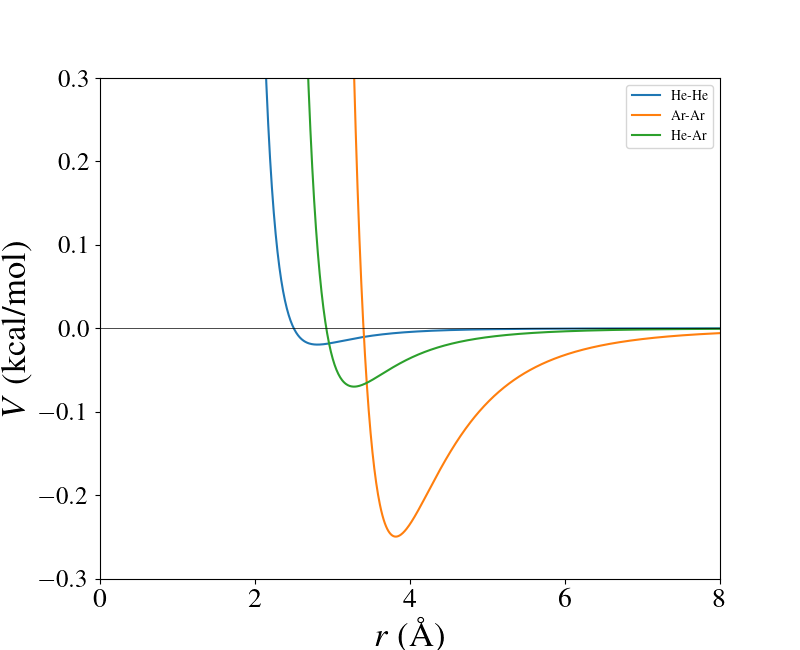
\includegraphics[width = .35\paperwidth]{media_paper/all_lj.png}
        \captionof{figure}{The interparticle potentials for He-He, Ar-Ar, and mixed Ar-He interactions are plotted against particle radius. 
        The potentials use the Leonard-Jones model (\ref{eq_6-12_pot}) for the parameter values given in Table \ref{tb_lj_diff}.
        }
        \label{fg_lj_all}
    \end{minipage}

\end{table}



\subsection{Parameter Estimation} \label{ssec_diff_estim}

The MD trajectories give the positions of each Argon (and Helium) atom at a sequence of discrete timesteps. 
We use a binning process to generate a space discretized approximation of the density of Argon at each timestep \cite{larson_1997_hydrodynamics}.
Let $N$ be the course-graining parameter of this binning.
In analogy to the difference equation, we use
\begin{equation}
    U_j^n\quad j\in[N]^d,\quad n=0,1\ldots,n_\text{max}
\end{equation}
to approximate the density of Argon at point $x=jh$ of timestep $n$.
We fit the data $U_j^n$ to the numerical approximation of the continuum model using a least squares error scheme.
The residuals are given by
\begin{equation} \label{eq_residuals}
    \{U_j^n-u_j^n(D)~\big|~0\le n\le n_\text{max},j\in[N]^d\}
\end{equation}
where $u_j^n(D)$ solves (\ref{ds_HE_CN}) for diffusion coefficient $D$ and initial condition $U_j^0$.
Solving this nonlinear optimization problem gives an estimate $\hat D$ of the diffusion coefficient.

In the implementation of the fitting algorithm, we used optimization routine $\texttt{curve\_fit}$ from the Python package $\texttt{scipy}$ \cite{scipy}.
This function takes a procedure parameter $f(D)$. 
The argument function $f(D)$ takes a prospective parameter value $D$ and returns the list of residuals.
The optimization function returns the parameter value $\hat D$ that minimizes the $L^2$ cost of the residuals returned by $f(\hat D)$, using the Levenberg-Marquardt algorithm.
Each iteration of the optimization procedure calls the input function $f$ on the prospective parameter value. 
To generate the residuals (\ref{eq_residuals}), $f$ runs the implicit scheme (\ref{ds_HE_CN}) for the given diffusion coefficient.
Even though the explicit scheme (\ref{ds_HE_FD}) is faster, we use the implicit scheme in the estimation procedure to avoid possible stability issues with exploring the parameter space.

\section{Results} \label{sec_diff_res}

We show results for two-dimensional simulations of molecular dynamics and continuum diffusion, although the algorithms are easily extended to three dimensions.
We impose periodicity on the MD domain boundary, matching the differential equation's boundary conditions. 
We conducted three LAMMPS simulations of Argon diffusion in Helium. 
Selected snapshots of the MD trajectory are shown in Figure \ref{fg_diff_results}.
The MD simulation box was 50000 \r{A} $\times$ 50000 \r{A}.
For simplicity, we use a dimensionless length scale where the unit square represents this domain.
There were 30000 helium atoms and 30000 argon atoms.
Each simulation proceeds from a unique pseudo-random initial condition.
The initial conditions were characterized by a uniform distribution of Helium in the simulation domain $[0,1]^2$ and a uniform distribution of Argon in $[1/4,3/4]^2$.
The particles were imbued with initial velocities satisfying the Maxwell-Boltzmann distribution of velocities for $T=300.00$ K. 
The pressure of the system was .995 atm.
The MD timestep was $k_\text{MD}=5$ fs. 
The repulsive term of the Leonard-Jones potential necessitates a small timestep for the integrator to be accurate.
The pairwise interaction range cutoff was $r_c=20$ \r{A}.
Each MD simulation was run for 1e6 timesteps. 

From each simulation, we use the procedure outlined in Section \ref{ssec_diff_estim} to estimate the diffusion coefficient $D$ of Argon. 
To reduce computational complexity, we use a larger timestep $k=1000k_\text{MD}$ for the difference equation model and only consider every 1000 MD timesteps. 
This gives $n_\text{max}=1000$ in (\ref{eq_residuals}).
The estimation procedure generates an estimate $\hat D_N$ for each binning precision $N=20,50,100$.
The result of solving the diffusion equation for $\hat D_{50}$ and $N=50$ is shown alongside the estimated order parameter with binning precision of 50 in Figure \ref{fg_diff_results}.
Table \ref{tb_diff_data} shows the error of solving the diffusion equation for each estimated parameter value at the different spatial precisions.

It is not surprising that the relative error decreases with higher resolution.
We expect the order parameter estimation to better represent the true system for large $N$.
The difference scheme accuracy (relative to the true solution) increases with $N$, which could contribute to this observation.
When $N$ is large enough however, the finite number of MD particles makes the estimated order parameter display the non-continuum effects.
Based on these competing effects, we expect there to be an optimal level of the binning resolution to achieve the greatest prediction accuracy.
This parameter depends on the size of the MD system, the number of particles, and their density.

While the relationship between binning resolution and error was expected, we did not anticipate its effect on the value of $\hat D$.
The variation in $\hat D$ between $N=20,50,$ and 100 is significant.
We don't see any reason for the estimated value to depend on the spatial resolution. 
It is interesting that this occurred in each MD run, and more experiments over a higher range of resolutions should be used to investigate this trend.

Other limitations of our approach that should be addressed in future experiments include:
\begin{itemize}
    \item We chose to use a continuum idealization of the initial condition when solving the differential equations. How well does the parameter estimation converge and perform when the MD initial condition is used?

    \item In some treatments of MD data as an order parameter, a convolution is used to smooth the approximation \cite{larson_1997_hydrodynamics}.
    Would a smoothing step prior to estimation help with the discrepancy across different binning resolutions?

    \item Does using the estimated diffusion coefficient have better prediction accuracy than the real diffusion coefficient for models based on the diffusion equation?

    \item With larger MD simulations and greater binning resolution, will the estimated diffusion coefficient approach the literature value?

    \item We used a linear approximation of the cost function to determine the confidence interval. With a nonlinear treatment of the confidence bands, would the the difference from literature be significant?
    
    \item Would the accuracy of the parameter estimation be improved with a higher order numerical scheme for the differential equation?
\end{itemize}


\begin{figure}[h]
    \centering
    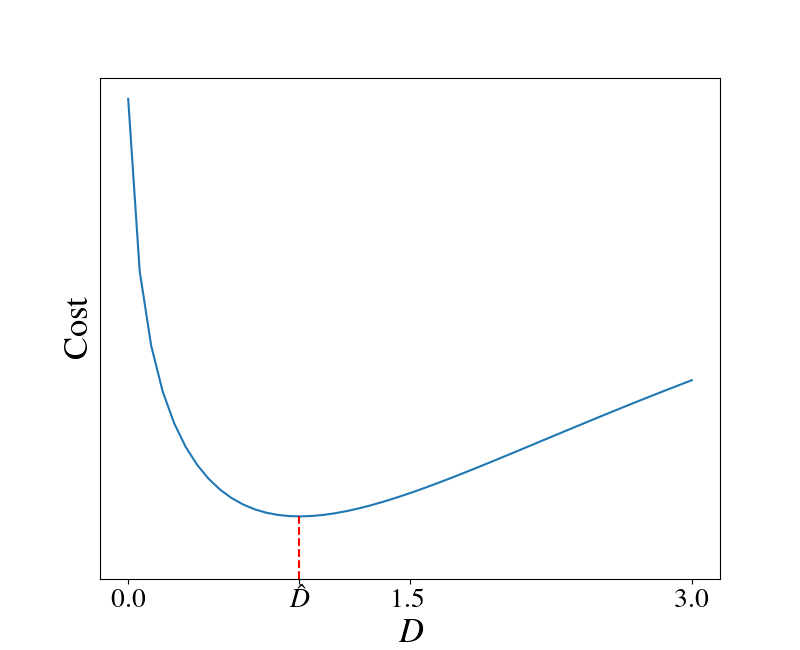
\includegraphics[width = .5\paperwidth]{media_paper/cost.png}
    \caption{The least squares error is plotted for values of $D$ near $\hat D$ when $N=20$.
    The unimodal shape of the plot suggests that a standard optimization procedure will estimate $\hat D$ accurately.}
    \label{fg_cost}
\end{figure}

\begin{table}[h] 
    \begin{tabular}{|l|l|l|l|l|l|}
        \hline
                   & $\hat D_N$ & $95\%$ CI & $N=20$ Error & $N=50$ Error & $N=100$ Error \\ \hline
        $N=20$     & 0.9121     & 0.0015    & 0.003223     & 0.002815     & 0.004819      \\ \hline
        $N=50$     & 0.7948     & 0.0005    & 0.003354     & 0.002821     & 0.004828      \\ \hline
        $N=100$    & 0.8417     & 0.0005    & 0.003292     & 0.002810     & 0.004819      \\ \hline
        Literature & 0.7335     & 0.0087    & 0.003455     & 0.002856     & 0.004852      \\ \hline
    \end{tabular}
\caption{We estimated diffusion coefficients for each MD run and binning precision. For each binning precision and estimated diffusion coefficient, we solved the heat equation with the finite difference method and calculated the difference from the order parameter estimated from MD. The error is averaged over the sampled time and space points.}
\label{tb_diff_data}
\end{table}

\begin{figure}[H]
% Cropping to 515 x 515 for MD, 670 x 650 for cmaps, 630 x 570 for surfs
% Top left: 250 x 250 for MD, 290 x 92 for cmaps, 370 x 135 for surfs

% mogrify -auto-orient -format png *.tga

% for f in cmap*1000*; do convert "$f" -crop 820x670+290+92 "end_$f" ; done ; for f in cmap*; do convert "$f" -crop 650x660+270+92 "$f" ; done

% for f in surf*1000*; do convert "$f" -crop 740x570+370+135 "end_$f" ; done ; for f in surf*; do convert "$f" -crop 630x570+335+135 "$f" ; done

    \def\subheight{.115\paperwidth}
    \centering
    \begin{tabular}{rccccc}

        ~ & $n=0$ & $n=50$ & $n=200$ & $n=500$ & $n=1000$ \\
        
        MD: &
        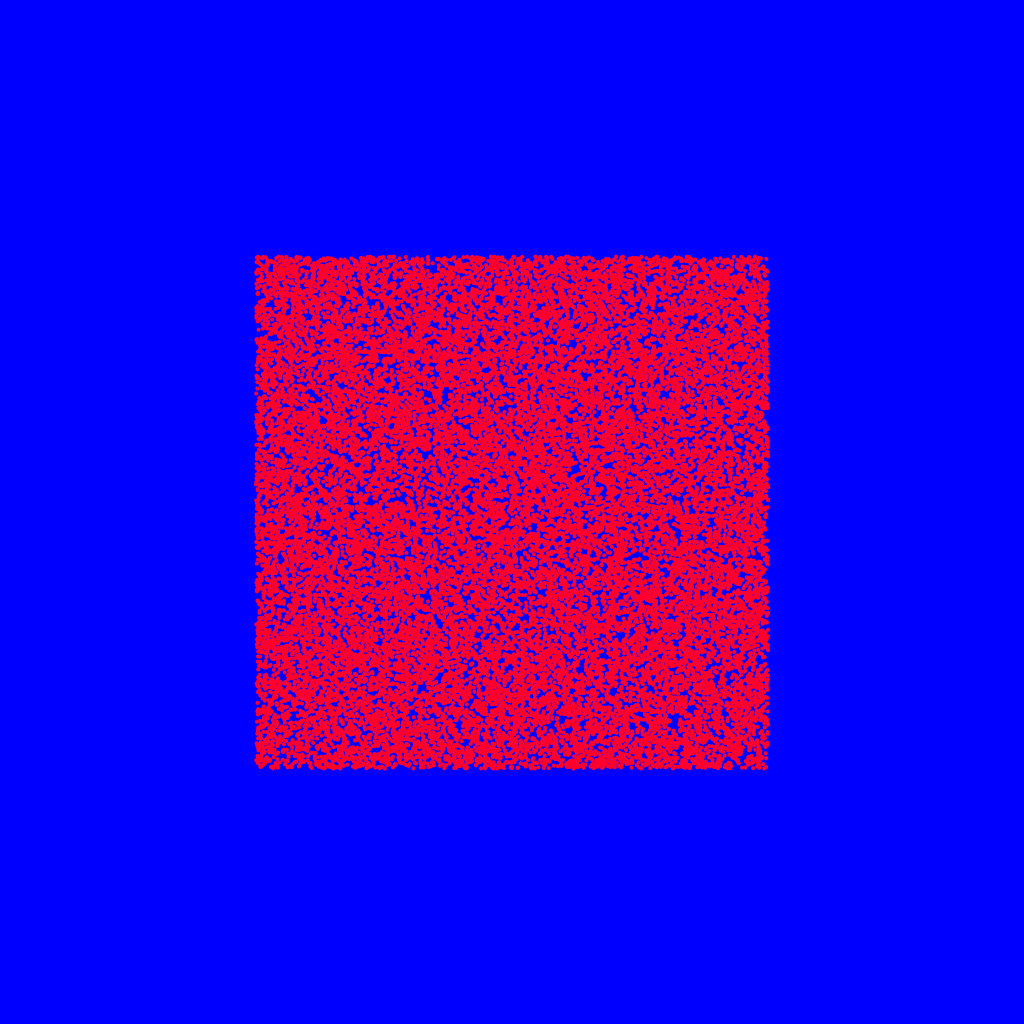
\includegraphics[align = c, height=\subheight]{media_paper/diff0.png} & 
        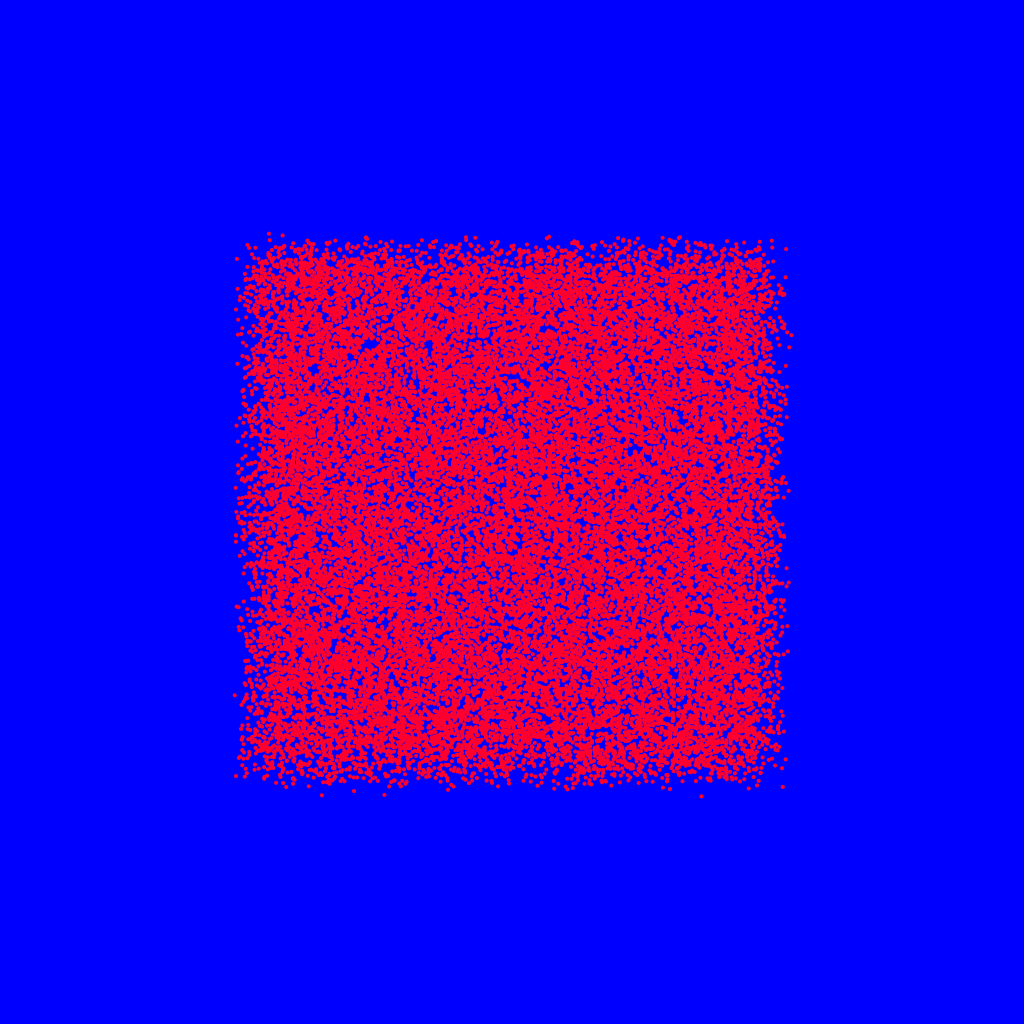
\includegraphics[align = c, height=\subheight]{media_paper/diff50.png} & 
        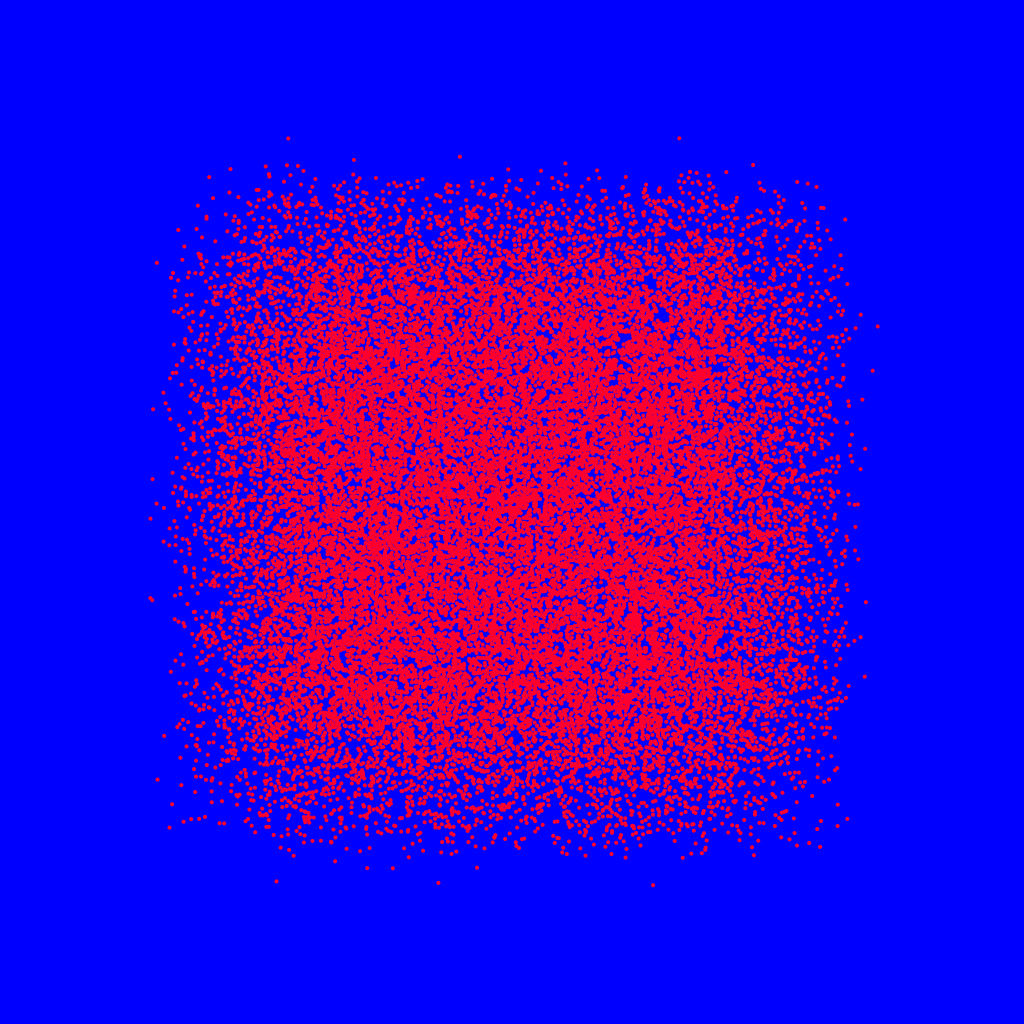
\includegraphics[align = c, height=\subheight]{media_paper/diff200.png} & 
        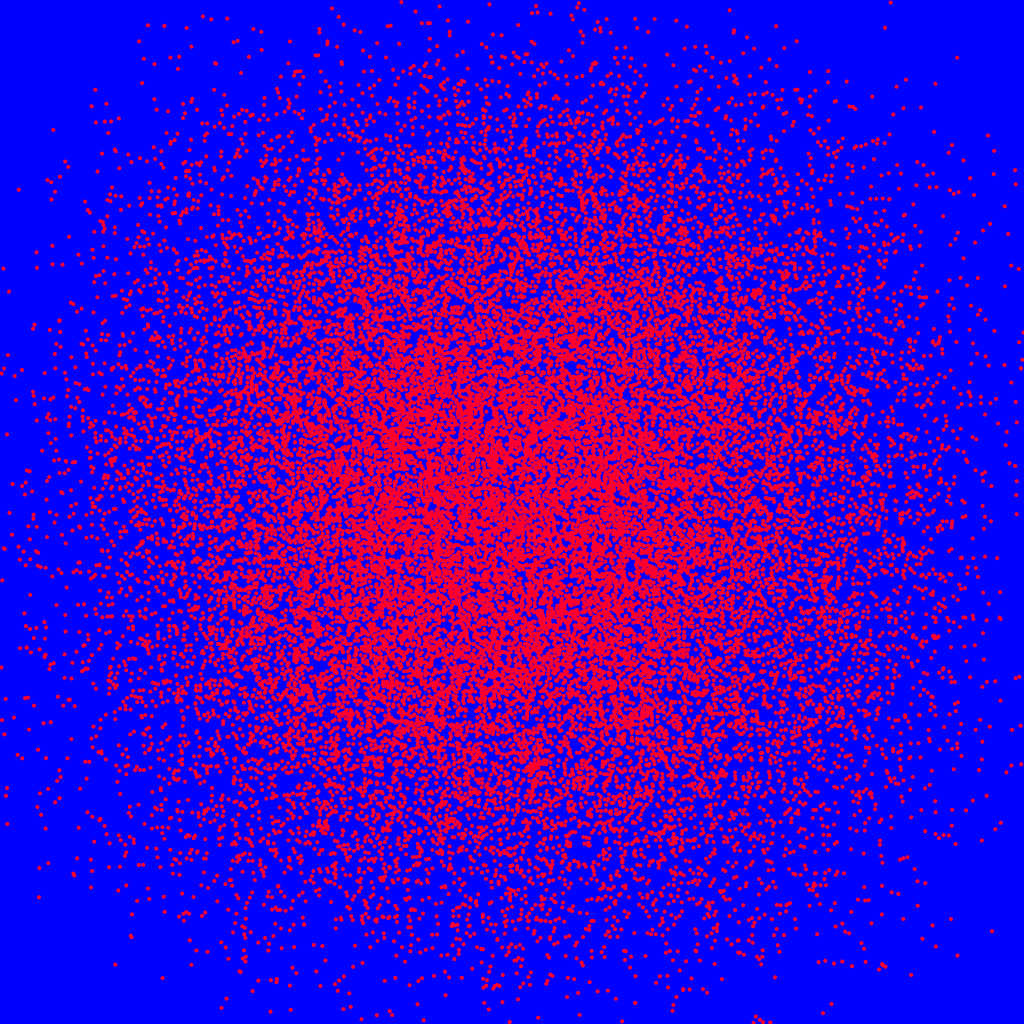
\includegraphics[align = c, height=\subheight]{media_paper/diff500.png} & 
        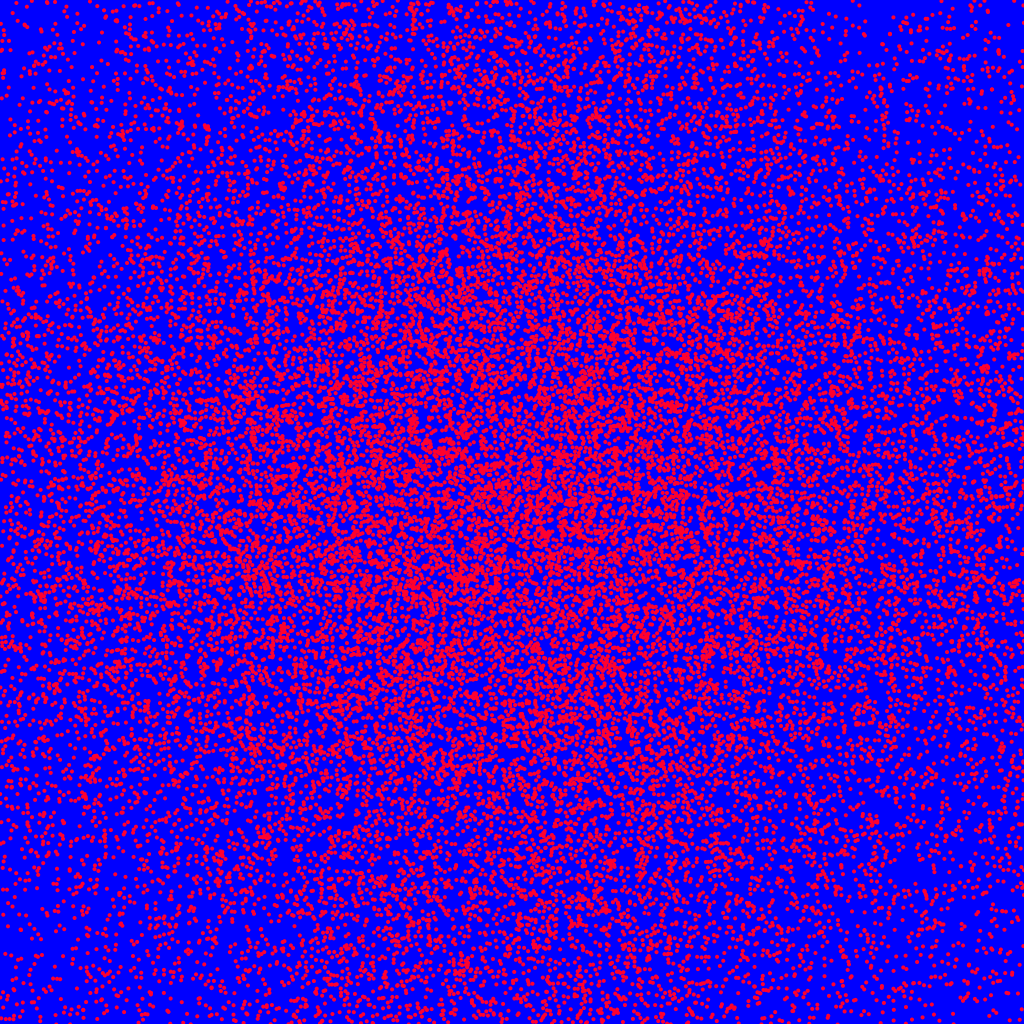
\includegraphics[align = c, height=\subheight]{media_paper/diff1000.png} \\

        MD: & 
        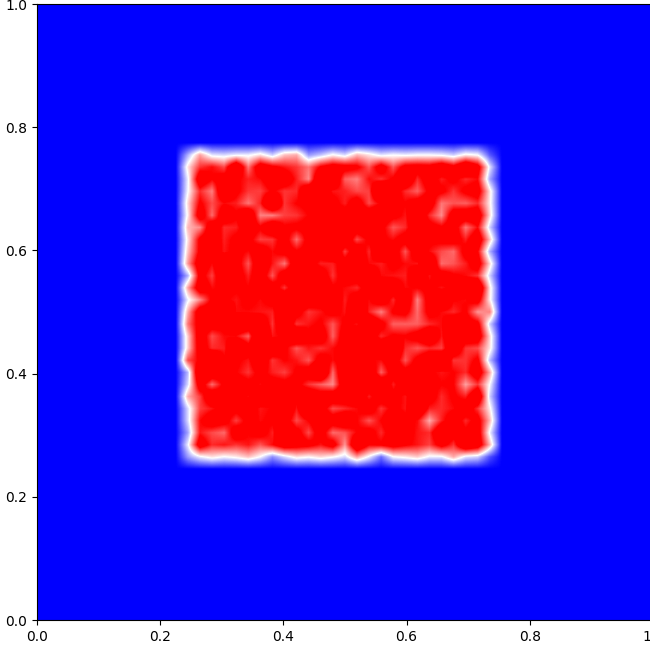
\includegraphics[align = c, height=\subheight]{media_paper/cmap_MD_n=0.png} & 
        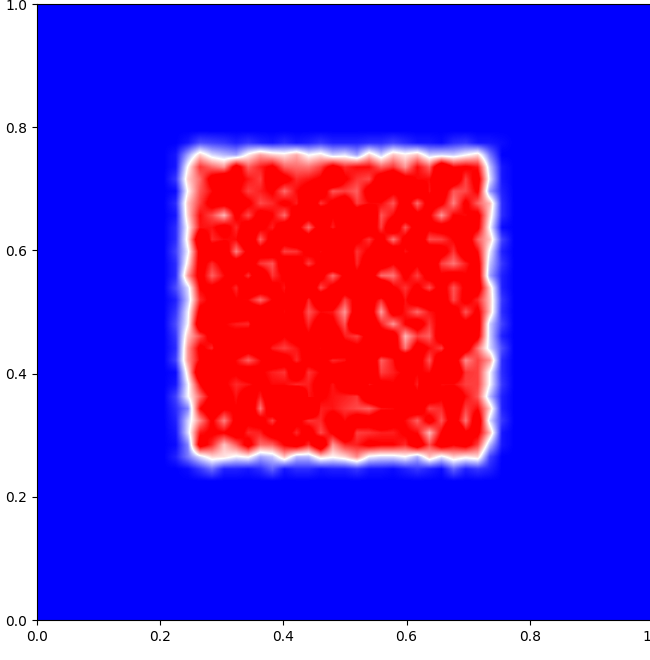
\includegraphics[align = c, height=\subheight]{media_paper/cmap_MD_n=50.png} & 
        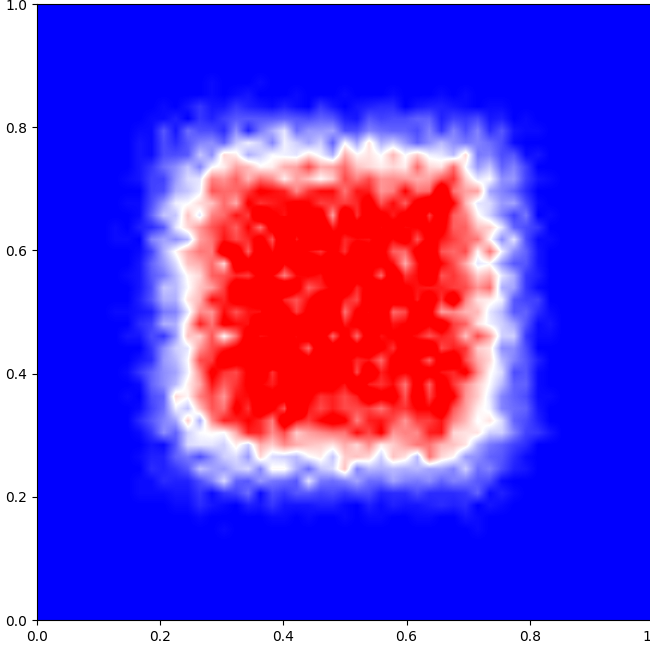
\includegraphics[align = c, height=\subheight]{media_paper/cmap_MD_n=200.png} & 
        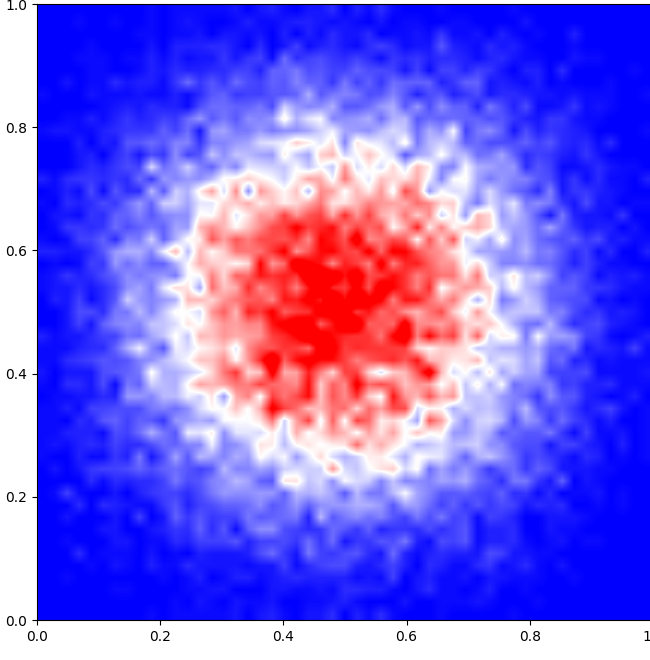
\includegraphics[align = c, height=\subheight]{media_paper/cmap_MD_n=500.png} & 
        % 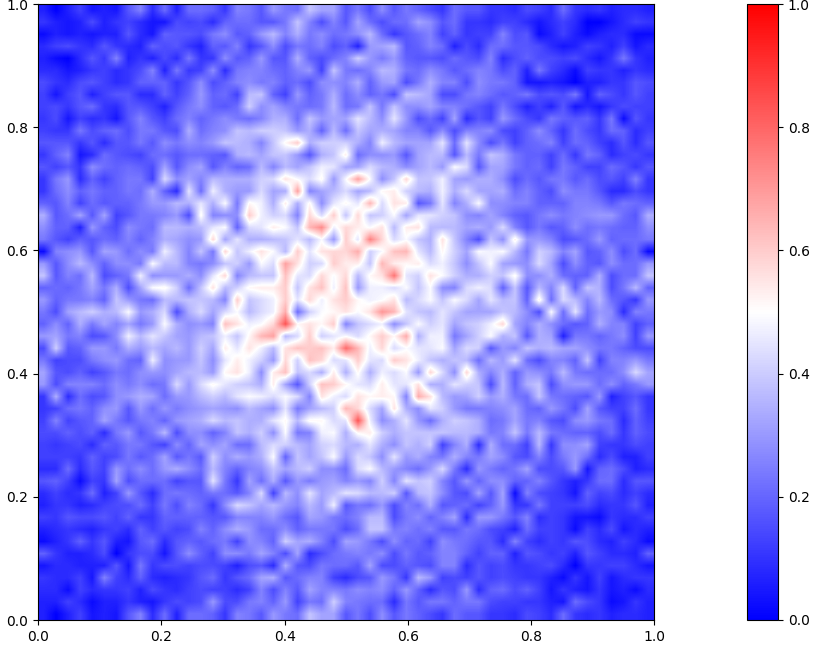
\includegraphics[align = c, height=\subheight]{media_paper/end_cmap_MD_n=1000.png} \\
        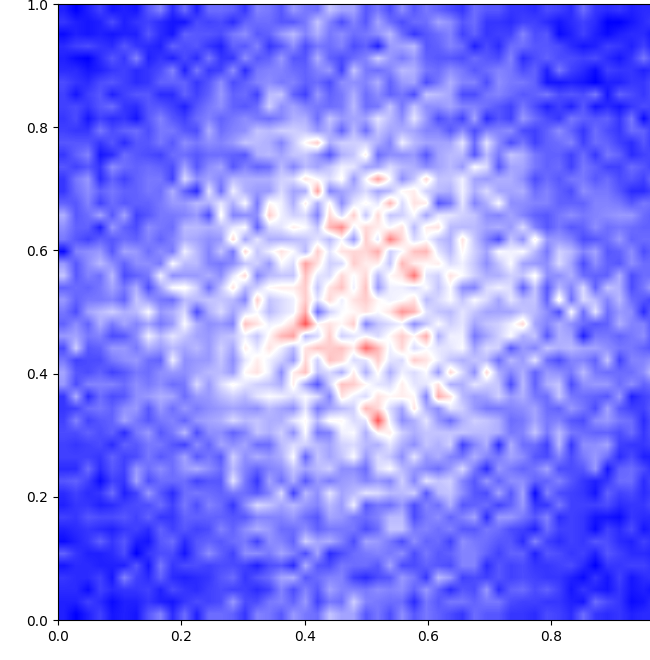
\includegraphics[align = c, height=\subheight]{media_paper/cmap_MD_n=1000.png} \\

        FD: &
        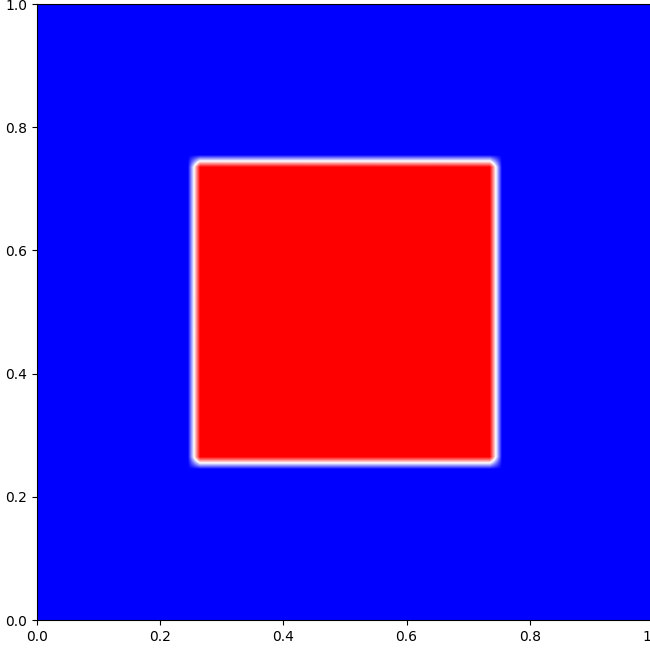
\includegraphics[align = c, height=\subheight]{media_paper/cmap_FD_n=0.png} & 
        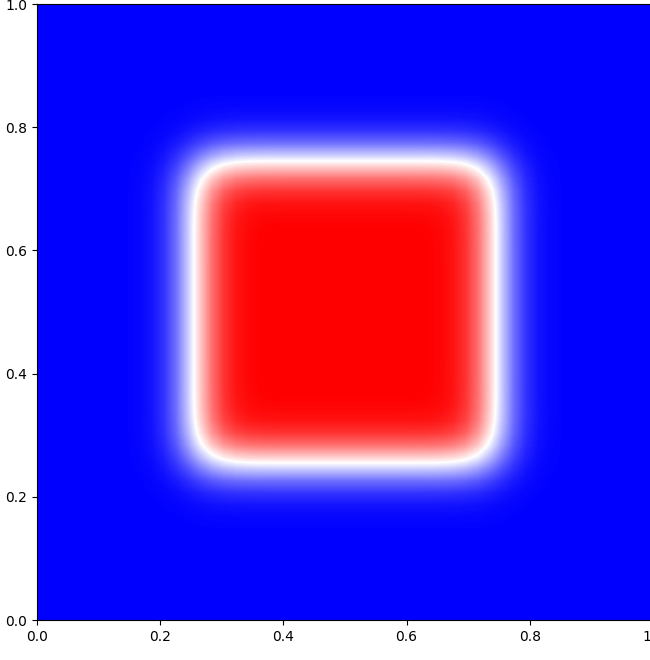
\includegraphics[align = c, height=\subheight]{media_paper/cmap_FD_n=50.png} & 
        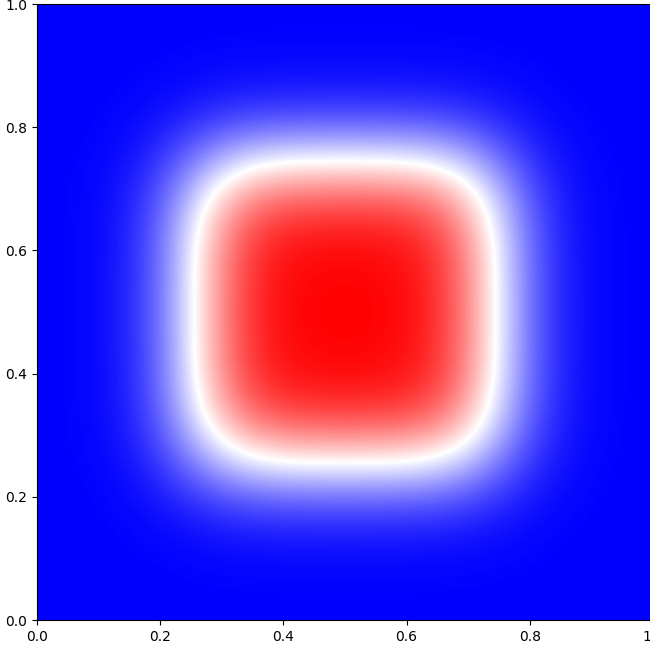
\includegraphics[align = c, height=\subheight]{media_paper/cmap_FD_n=200.png} & 
        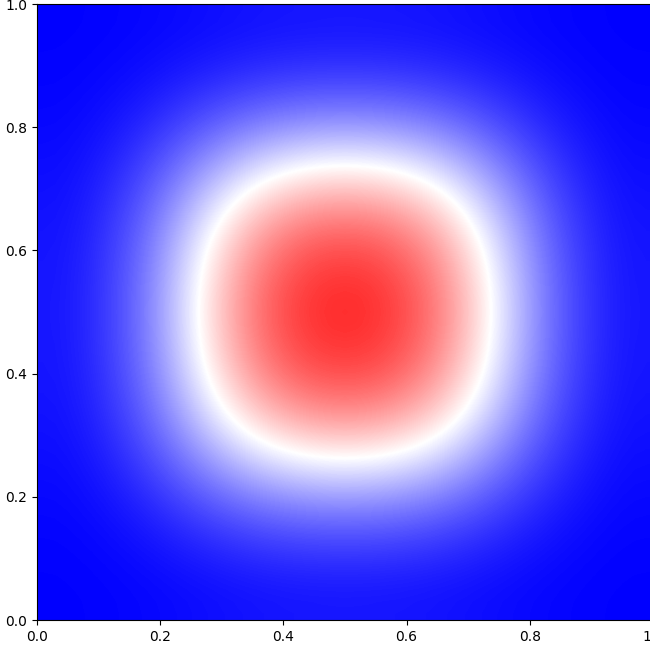
\includegraphics[align = c, height=\subheight]{media_paper/cmap_FD_n=500.png} & 
        % 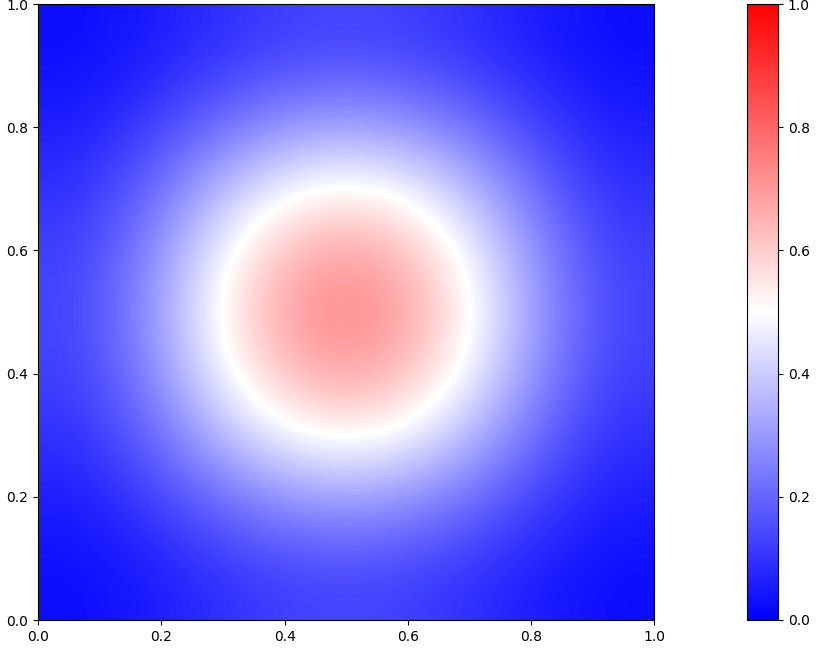
\includegraphics[align = c, height=\subheight]{media_paper/end_cmap_FD_n=1000.png} \\
        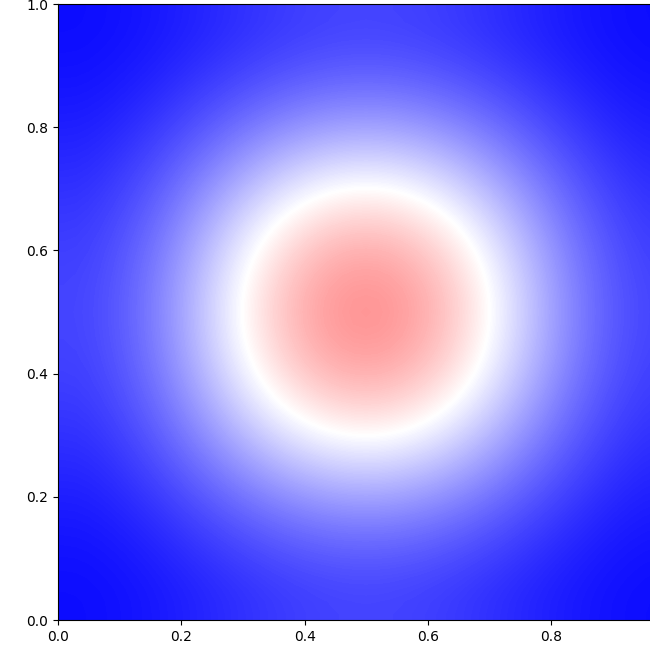
\includegraphics[align = c, height=\subheight]{media_paper/cmap_FD_n=1000.png} \\

        MD: &
        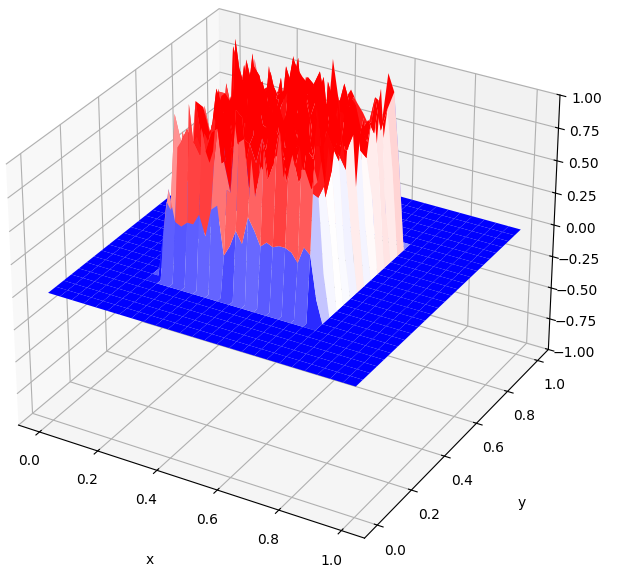
\includegraphics[align = c, height=\subheight]{media_paper/surf_MD_n=0.png} &
        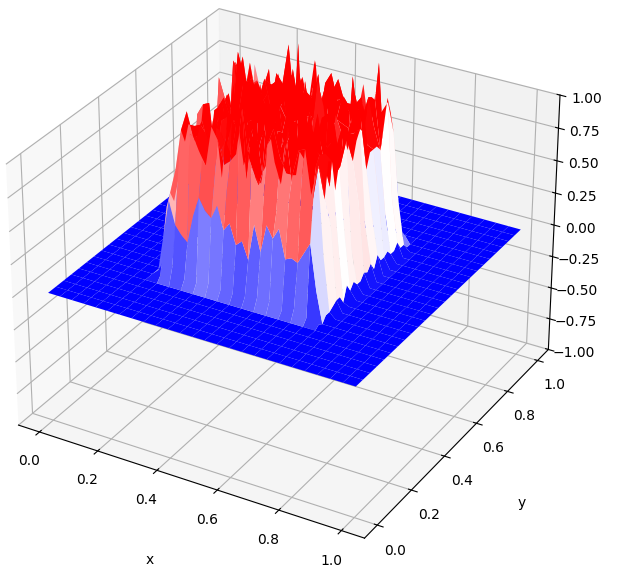
\includegraphics[align = c, height=\subheight]{media_paper/surf_MD_n=50.png} &
        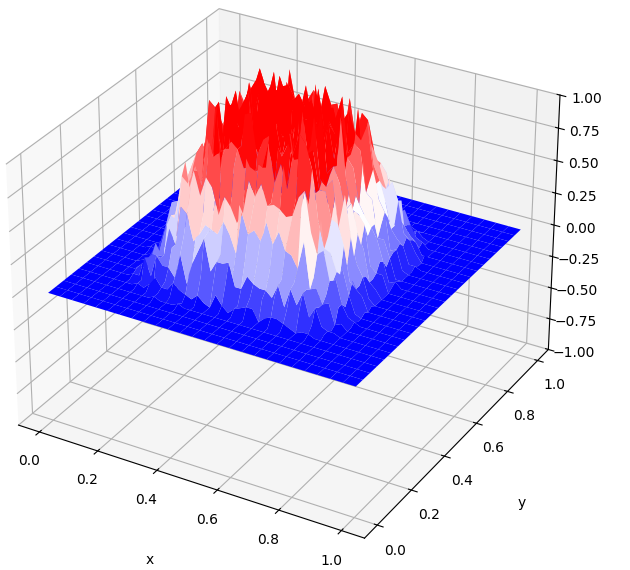
\includegraphics[align = c, height=\subheight]{media_paper/surf_MD_n=200.png} &
        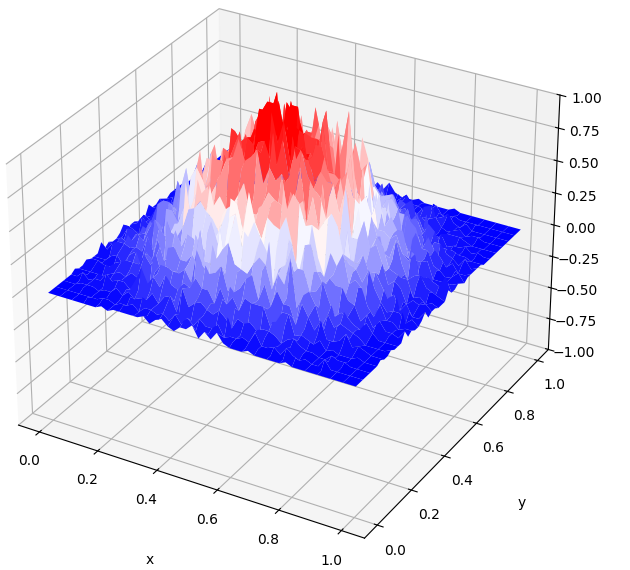
\includegraphics[align = c, height=\subheight]{media_paper/surf_MD_n=500.png} &
        % 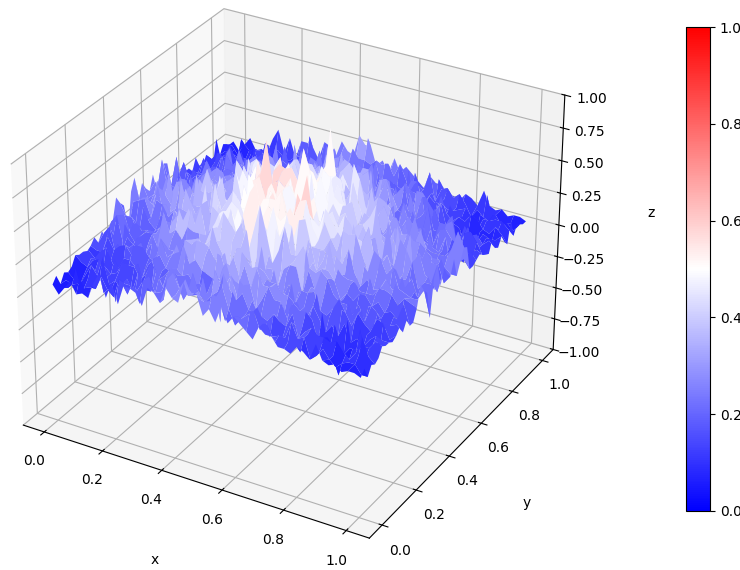
\includegraphics[align = c, height=\subheight]{media_paper/end_surf_MD_n=1000.png} \\
        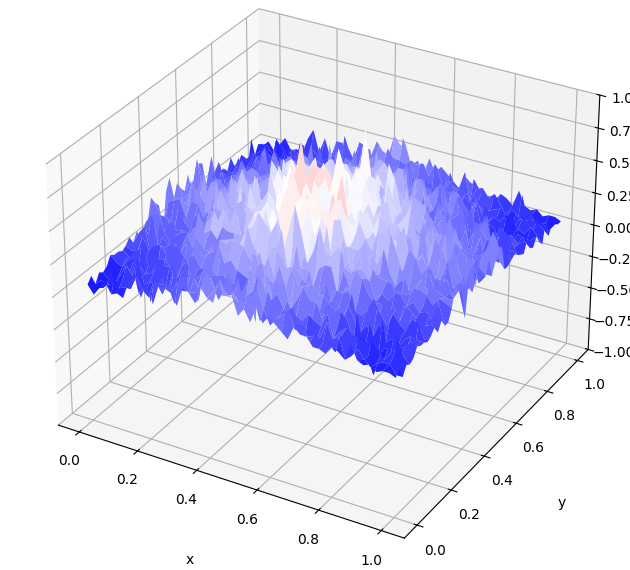
\includegraphics[align = c, height=\subheight]{media_paper/surf_MD_n=1000.png} \\

        FD: &
        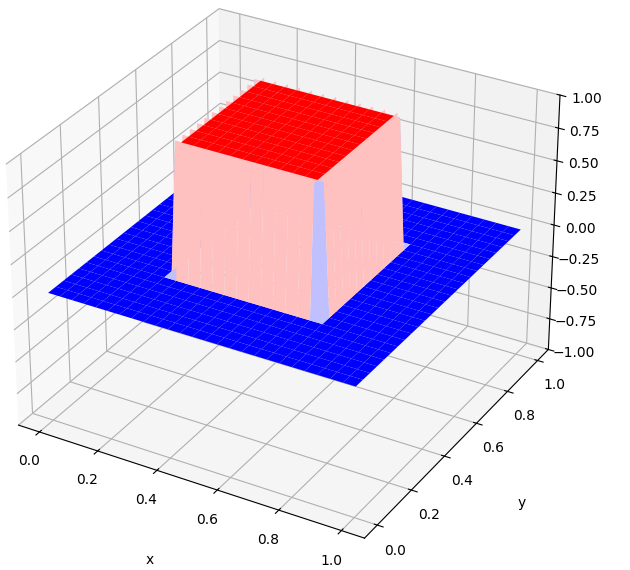
\includegraphics[align = c, height=\subheight]{media_paper/surf_FD_n=0.png} &
        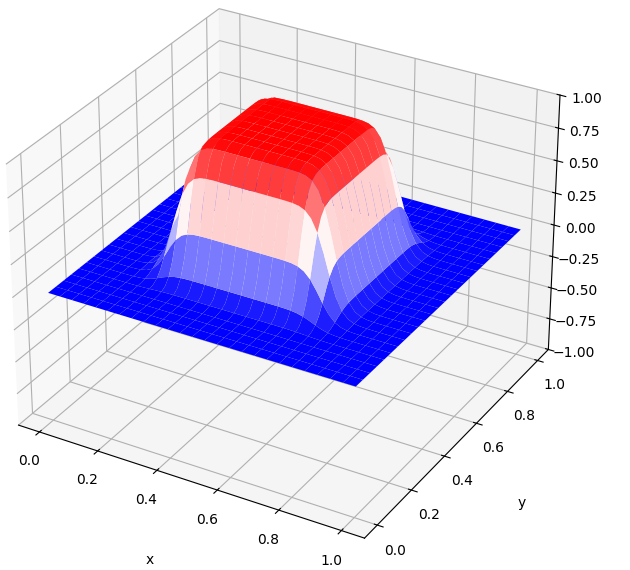
\includegraphics[align = c, height=\subheight]{media_paper/surf_FD_n=50.png} &
        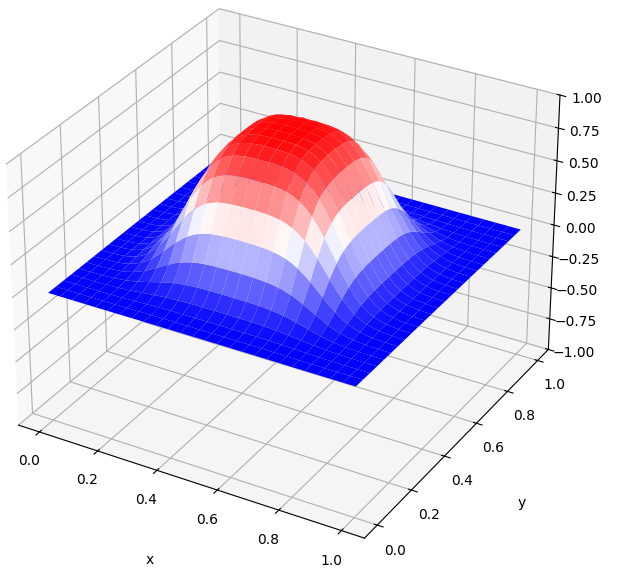
\includegraphics[align = c, height=\subheight]{media_paper/surf_FD_n=200.png} &
        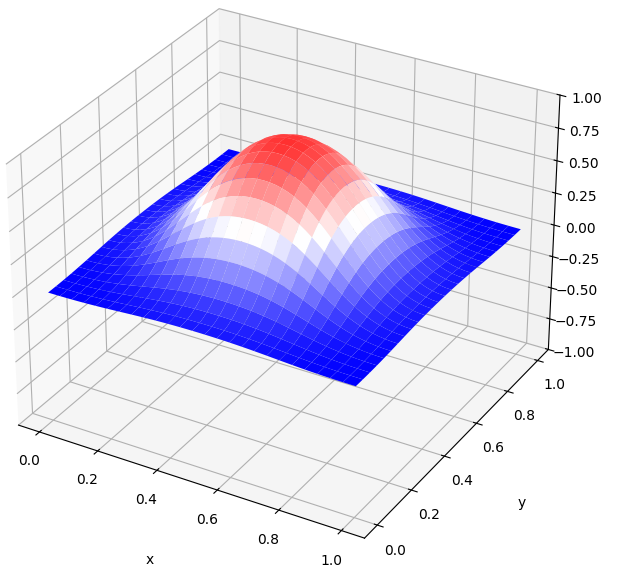
\includegraphics[align = c, height=\subheight]{media_paper/surf_FD_n=500.png} &
        % 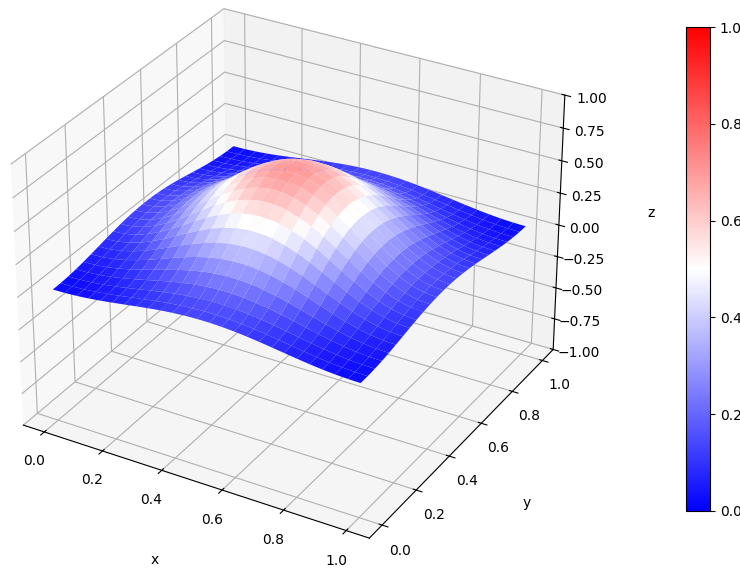
\includegraphics[align = c, height=\subheight]{media_paper/end_surf_FD_n=1000.png}
        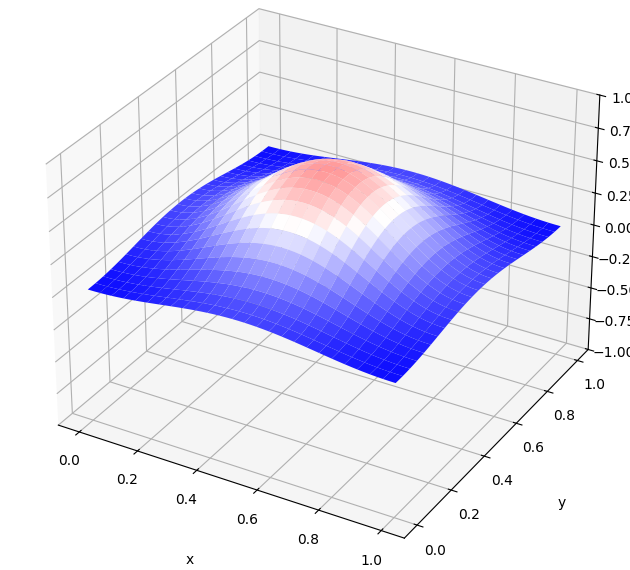
\includegraphics[align = c, height=\subheight]{media_paper/surf_FD_n=1000.png}
    \end{tabular}

    \hspace{40pt}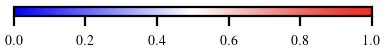
\includegraphics[width = .55\paperwidth]{media_paper/diff_colorbar.png}

    \caption{ % PUT MD Parameters,BC here and in the text
        The initial condition for MD simulations was a uniform random concentration of Argon in $[1/4,3/4]^2$ and 0 outside. 
        The initial distribution of Helium was uniform in $[0,1]^2$.
        The initial condition for the heat equation was 1 in $[1/4,3/4]^2$ and 0 outside.
        The order parameters were both scaled to mean $1/4$ for presenting the data.
        In the figure, the fitting results are shown for a binning parameter of $N=50$. 
        Columns 1-5 display timesteps $n=0,50,200,500,1000$, respectively.
        On the top row, MD snapshots are shown.
        In the second and fourth row, the order parameter estimated from the MD trajectory is shown.
        In the third and fifth row, the solution to the heat equation for the parameter $\hat D_{50}$ with spatial resolution $N=50$ and appropriate initial condition is shown.
    }
    \label{fg_diff_results}
\end{figure}


\chapter{Phase Separation} \label{sec_phase}

\begin{wrapfigure}{r}{.4\paperwidth}
    \centering
    \vspace{-30pt}
      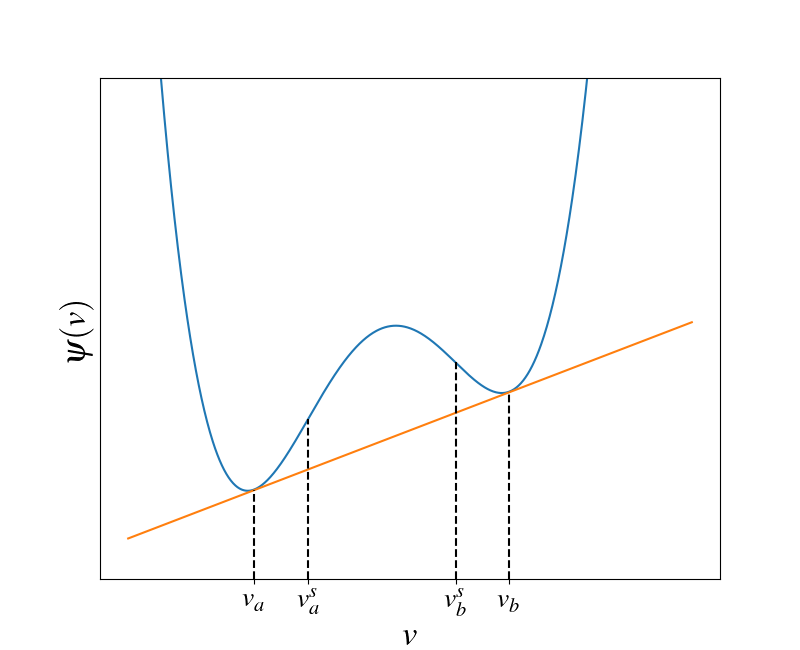
\includegraphics[width=.4\paperwidth]{media_paper/gen_well}
      \captionof{figure}{The phase energy is represented by a double well potential. Here we show a general double well potential. The points $v_a$ and $v_b$ are the local minima of $\psi$. $v_a^s$ and $v_b^s$ share the orange supporting tangent.}
      \label{fg_gen_well}
\end{wrapfigure}
Chemical phase separation occurs in some multicomponent systems when the mixture separates into regions of the pure components.
We consider a two component mixture of fluids.
Here, the order parameter $v$ is the difference in mole fractions of the components.
At high temperature, the system exists at equilibrium as a homogeneous phase.
When cooled below a critical temperature, phase separation may begin.
Below this critical temperature, the Ginzburg-Landau free energy of the system takes a double well shape.
This function $\psi:[-1,1]\to\mathbb{R}$ is graphed in Figure \ref{fg_gen_well}. 

The curvature of $\psi$ defines the stability properties of phases. 
Below the critical temperature, the order parameter lies in one of three regions \cite{copetti_1990_kinetics}, \cite{novickcohen_1984_nonlinear}. 
In the unstable, or spinodal, region, $\psi''(v)<0$.
The points $v_a^s$ and $v_b^s$ where $\psi''=0$ are called the spinodal points. 
Inside $(v_a^s,v_b^s)$, any fluctuations in the order parameter are unstable, growing into separation.
In the metastable region, phase separation proceeds by nucleation. 
Small fluctuations in the order parameter may increase energy, but sufficiently large perturbations grow in time. 
The binodal points $v_a$ and $v_b$ where the supporting tangent lines touches are shown in Figure \ref{fg_gen_well}.
The metastable region is defined precisely as $(v_a,v_a^s)\cup(v_b^s,v_b)$.
Outside the metastable region, $v$ is stable and all fluctuations increase the phase energy.

\begin{wrapfigure}{l}{.4\paperwidth}
    \centering
    \vspace{-15pt}
    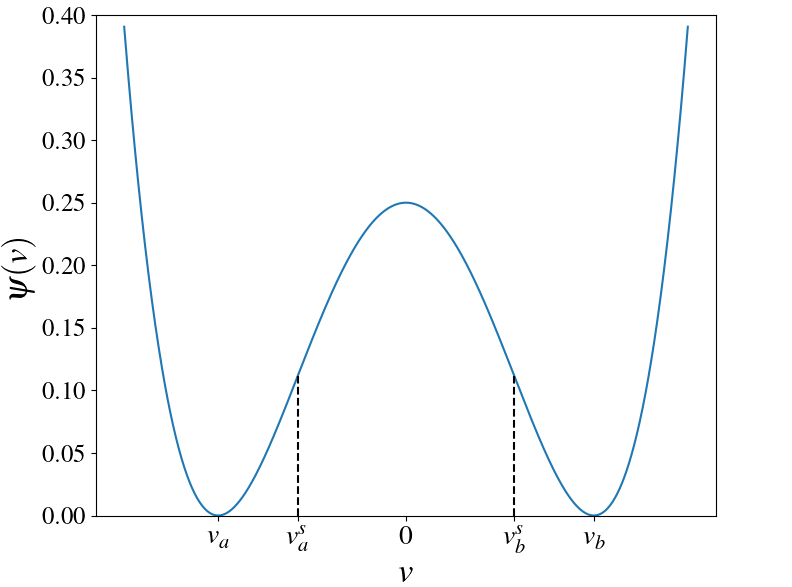
\includegraphics[width=.4\paperwidth]{media_paper/our_well}
    \captionof{figure}{Our chosen phase energy function (\ref{eq_double_well}). Here, $v_a=-1$, $v_a^s=-\frac{1}{\sqrt{3}}$, $v_b^s=\frac{1}{\sqrt{3}}$, and $v_b=1$.}
  \label{fg_double_well} 
\end{wrapfigure}
It is common to approximate $\psi$ as a quartic polynomial \cite{novickcohen_1984_nonlinear}.
For our differential equation models, we can restrict our attention to symmetric $\psi$. 
\cite{copetti_1990_kinetics} show that any quartic $\psi$ reduces to solving the equation for a free energy function of the form
\begin{equation} \label{eq_gen_psi}
    \psi(v )=\frac{\alpha}{4}(v^2-\beta^2)^2.
\end{equation}
For numerical results, we will use the specific potential
\begin{equation} \label{eq_double_well}
    \psi(v )=\frac{1}{4}(v^2-1)^2
\end{equation}
shown in Figure \ref{fg_double_well}. 
For this $\psi$, the spinodal region is $(-\frac{1}{\sqrt{3}},\frac{1}{\sqrt{3}})$ and the metastable region is $(-1,-\frac{1}{3})\cup(\frac{1}{3},1)$. 
The only stable points are the pure phases 1 and -1.


\section{Gradient Flow Equations} \label{sec_func}

\subsection{Phase Energy Functional}

Using the general Ginzburg-Landau free energy $\psi$, Cahn and Hilliard propose an energy functional 
\begin{equation} \label{eq_func}
    F(u)=M\int_{\Omega}\psi(u)+ \frac{\gamma}{2}|\nabla u|^{2}~dx
\end{equation}
describing phase separation \cite{cahn_1958_free}.
For a configuration described by $u$, $F(u)$ is the total free energy of the system. 
The term $\int\psi$ represents the energy associated with a homogeneous system.
Since $\psi$ attains its minimal value at the pure phases, the first term of (\ref{eq_func}) favors separation.
The second term $\int\frac{\gamma}{2}|\nabla u|^2$ is entropic.
It handles the non-uniformity of the system by associating energy with the magnitude of the concentration gradient.
This makes large concentrations gradients energetically unstable and introduces the diffusive dynamics that should be present in any fluid.
The parameter $\gamma$ determines the relative scale of diffusive and separation forces.
Physically, this determines the interface distance between pure phases.
A larger $\gamma$ corresponds to stronger diffusion and a wider interface.

A variational approach provides a necessary condition on functions $u$ which minimize $F$. Setting 
\begin{equation} \label{eq_def_f}
    f(x,u,\nabla u)=\psi(u)+ \frac{\gamma}{2}|\nabla u|^{2}
\end{equation}
gives the Euler-Lagrange equation for $F$ as
\begin{equation} \label{eq_EL1}
    \frac{\partial f}{\partial u}-\sum_{n=1}^{d}\frac{\partial }{\partial x_{n}}\frac{\partial f}{\partial u_{x_{n}}}=0,
\end{equation}
or equivalently
\begin{equation} 
    \frac{\partial f}{\partial u}-\nabla_{x}\cdot\nabla_{u_{x}}f=0.
\end{equation}
From (\ref{eq_def_f}), we have
\begin{equation} 
    \frac{\partial f}{\partial u_{x_{n}}}=\gamma\frac{\partial u}{\partial x_{n}},
\end{equation}
so
\begin{equation} 
    \nabla_{x}\cdot\nabla_{u_{x}}f=\gamma\nabla^{2}u
\end{equation}
and 
\begin{equation} 
    \frac{\partial f}{\partial u}=\psi'(u)=\phi(u).
\end{equation}
Therefore, the Euler-Lagrange equation is 
\begin{equation} \label{eq_EL}
    \phi(u)-\gamma\nabla^{2}u=0.
\end{equation}

Any equilibria of the system with energy $F$ should satisfy (\ref{eq_EL}). 
We can use a gradient flow to introduce time evolution towards this minimal energy state.
Gradient flow equations use the Fr\'echet derivative of an energy functional to decrease the system energy over time.

Let $\mathcal{F}$ be a Hilbert space with inner product $(\cdot ~, \cdot)_{\mathcal{F}}$ and induced norm $\|\cdot\|_{\mathcal{F}}$.
For an energy functional $F:\mathcal{F }\to\mathbb{R}$, the Fr\'echet derivative at a point $u\in\mathcal{F}$ is the unique linear operator $\frac{\partial F}{\partial u}$ satisfying
\begin{equation}
    \langle \frac{\partial F}{\partial u},v\rangle=\lim_{\epsilon\to0}\frac{\ud}{\ud\epsilon}F(u+\epsilon v)\bigg|_{\epsilon=0}.
\end{equation}
Using the Riesz Representation theorem, we associate
\begin{equation}
    \langle \frac{\partial F}{\partial u},v\rangle = (\frac{\partial F}{\partial u},v)_{\mathcal{F}}.
\end{equation}
The gradient flow equation for $F$ follows as
\begin{equation} \label{eq_grad_flow}
    \frac{\partial u}{\partial t}=-\kappa\frac{\partial F}{\partial t},
\end{equation}
where $\kappa>0$ is a constant scaling time. From the functional chain rule, we have 
\begin{equation*}
    \frac{\ud}{\ud t}F(u)=(\frac{\partial F}{\partial u},\frac{\partial u}{\partial t})_{\mathcal{F}}=(\frac{\partial F}{\partial u},-\kappa\frac{\partial F}{\partial u})_{\mathcal{F}}=-\kappa\left\|\frac{\partial F}{\partial u}\right\|_{\mathcal{F}}^2\le0.
\end{equation*}
This shows that (\ref{eq_grad_flow}) has the desirable physical property of the system's total energy decaying in time.

\subsection{Function Spaces}

We will derive two differential equation models as gradient flows of the phase energy functional (\ref{eq_func}). First, we introduce the function spaces for differentiation. 
The space
\begin{equation} \label{eq_l2space}
    L^{2}(\Omega,\mathbb{R}^{d}):=\left\{f\colon \Omega\to \mathbb{R}^{d}~\bigg|~\int_{\Omega}|f(x)|^{2}~dx<\infty\right\}
\end{equation}
of square integrable functions has inner product
\begin{equation} \label{eq_l2ip}
    ( f,g)_{2}:=\int_{\Omega}f(x)\cdot g(x)~dx
\end{equation}
and induced norm 
\begin{equation} \label{eq_l2norm}
    \|f\|_{2}=\sqrt{( f,f)_{2}}=\left(\int_{\Omega}|f(x)|^{2}\ dx\right)^{\frac{1}{2}}.
\end{equation}
For $L^2$ functions $f$ and $g$, we have a useful identity for the norm of their sum
\begin{equation}\label{eq_l2normsum}
    \begin{split} 
        \|f+g\|_{2}^{2}&=\int_{\Omega}|f(x)+g(x)|^{2}~dx\\
        &=\int_{\Omega}|f(x)|^{2}+2f(x)\cdot g(x)+|g(x)|^{2}~dx\\
        &=\|f\|^{2}_{2}+( f,g)_{2}+\|g\|^{2}_{2}.
    \end{split}
\end{equation}

To keep periodic boundary conditions consistent with the molecular dynamics model, we will consider a periodic subspace
\begin{equation} 
    L_{p}^{2}:=\left\{u\in L^{2}([0,1]^{d}):u\big|_{x_{i}=0}=u\big|_{x_{i}=1},1\le i\le d\right\}
\end{equation}
of $L^{2}$.
This is a Hilbert space under the $L^{2}$ inner product and norm. 

Sobolev spaces generalize $L^2$, introducing additional regularity by requiring derivatives to be square-integrable. Generally, the $L^{2}$ Sobolev spaces are defined by 
\begin{equation}
    H^{m}(\Omega)=\{u\in L^{2}(\Omega):\partial ^{\alpha}u\in L^{2}(\Omega)\text{ for all }|\alpha|\le n\}
\end{equation}
for non-negative integers $m$. 
$H^{m}(\Omega)$ is a Hilbert space with inner product 
\begin{equation} \label{eq_IP}
    (u,v)_{H^{m}}=\sum_{|\alpha|\le m}(\partial ^{\alpha}u,\partial ^{\alpha}v)_{2}
\end{equation}
and induced norm
\begin{equation} 
    \|u\|_{H^{m}}=\{(u,u)_{m}\}^{\frac{1}{2}}.
\end{equation}

Specifically considering functions on our spatial domain $\Omega=[0,1]^{d}$, we define the periodic Sobolev spaces
\begin{equation} 
    H^{m}_{p}=H^{m}([0,1]^{d})\cap L^{2}_{p}.
\end{equation}
To ensure uniqueness of solutions, we will further restrict our analysis to zero-average functions by defining
\begin{equation} 
    \dot H_{p}^{m}=\{u\in H^{m}_{p}:\int_{\Omega}u(x)~dx=0\}.
\end{equation}
We note that $H^{m}_{p}$ and $\dot H^{m}_{p}$ are Hilbert spaces under the same inner product (\ref{eq_IP}). 
Additionally, for functions $u,v\in\dot H^{m}_{p}$, the inner product becomes 
\begin{equation} 
    (u,v)_{H^{m}}=\sum_{1\le|\alpha|\le m}(\partial ^{\alpha}u,\partial ^{\alpha}v)_{2}.
\end{equation}

We extend these constructions to $m<0$ by defining 
\begin{equation} 
    H^{-m}(\Omega)=(H^{-m}(\Omega))^*.
\end{equation}
Similarly, extend $H^m_p$ and $\dot H^m_p$ to negative $m$ using their dual spaces.
The Riesz Representation theorem defines the inner product 
\begin{equation} \label{eq_IP_RRT}
    (u^{*},v^{*})_{H^{-m}}:=(u,v)_{H^m}
\end{equation}
on the dual spaces, where for each $u^{*},v^{*}\in H^{-m}(\Omega)$, $u,v\in H^{m}(\Omega)$ are their associates. 




\subsection{Allen-Cahn Derivation}

We derive the Allen-Cahn equation as the gradient flow of the phase energy function $F$ over $L^2_p$.
Begin by computing the linear approximation of $F$.
\begin{align} \label{eq_lin_approx}
    F(u+\epsilon v)&= M\int_{\Omega}\psi(u+\epsilon v)+ \frac{\gamma}{2}|\nabla u+\epsilon\nabla v|^{2}\ dx
\end{align}
Using (\ref{eq_l2normsum}), the second term of (\ref{eq_lin_approx}) may be written 
\begin{align}
        \int_{\Omega}|\nabla u+\epsilon\nabla v|^{2}\ dx&=\|\nabla u\|_{2}^{2}+2( \nabla u,\epsilon\nabla v)_{2}+\|\epsilon \nabla v\|_{2}^{2}\\
        &=\|\nabla u\|_{2}^{2}+2\epsilon(\nabla u,\nabla v)_{2}+\epsilon^{2}\|\nabla v\|_{2}^{2}.\label{eq_above}
\end{align}
To handle the inner-product term of (\ref{eq_above}) we note the following useful vector relationships 
\begin{align}
    \nabla u\cdot \nabla v&= \sum_{n=1}^{d}\frac{\partial u}{\partial x_{n}}\frac{\partial v}{\partial x_{n}}\\
    \nabla \cdot(u\nabla v)&= \sum_{n=1}^{d}\frac{\partial}{\partial x_{n}}\left(u \frac{\partial v}{\partial x_{n}}\right)\\
    &= \sum_{n=1}^{d} \frac{\partial u}{\partial x_{n}}\frac{\partial v}{\partial x_{n}}+\sum_{n=1}^{d}u\frac{\partial^{2} v}{\partial^{2} x_{n}}\\
    &= \nabla u\cdot \nabla v+u\nabla ^{2}v.
\end{align}
We have
\begin{equation} \label{eq_genIBP}
    \begin{split} 
    (\nabla u,\nabla v)_{2}&= \int_{\Omega}\nabla u\cdot \nabla v~dx\\
    &= \int_{\Omega}\nabla \cdot(v \nabla u)-v \nabla ^{2}u\ dx\\
    &= \underbrace{\int_{\partial \Omega}v\nabla u\cdot n~dx}_{=0\text{ by }(\ref{eq_below})}-\int_{\Omega}(\nabla ^{2}u)\cdot v~dx\quad(\text{Divergence Theorem})
    \\
    &= -(\nabla ^{2}u,v)_{2}.
    \end{split}
\end{equation}
We already have assumed that $u$ and $v$ are 1-periodic. If we additionally require that $\nabla u$ is periodic, 
\begin{equation} \label{eq_below}
    \begin{split}
        \int_{\partial\Omega}v\nabla u\cdot n~\ud x&=\sum_{i=1}^{d }\left\{\int_{[0,1]^{d-1}}v(x,t)\big|_{x_i=0}~\left[\nabla u(x,t)\big|_{x_i=0}\cdot -e_i\right]~\ud x\right.\\
        &+\left.
        \int_{[0,1]^{d-1}}v(x,t)\big|_{x_i=1}~\left[\nabla u(x,t)\big|_{x_i=1}\cdot e_i\right]~\ud x
        \right\}\\
    &=0
    \end{split}
\end{equation}
allowing us to set the boundary integral in (\ref{eq_genIBP}) to 0.

We can now compute the Fr\'echet derivative of $F$. First,
\begin{align}
    \frac{d}{d \epsilon}F(u+\epsilon v)&= \frac{d}{d \epsilon}\left[\int_{\Omega}\psi(u+\epsilon v)\ dx+\|u\|_{2}^{2}+\epsilon(-\nabla ^{2}u,v)_{2}+\epsilon^{2}\|v\|_{2}^{2}\right]\\
    &= \int_{\Omega} \frac{d}{d \epsilon}\psi(u+\epsilon v)~dx+(-\nabla ^{2}u,v)_{2}+2\epsilon \|v\|_{2}^{2}\\
    &= \int_{\Omega}\psi'(u+\epsilon v)\cdot v~dx+(-\nabla ^{2}u,v)_{2}+2\epsilon \|v\|^{2}_{2}
\end{align}
where we applied the Liebniz integration rule to bring $\frac{\ud}{\ud\epsilon}$ inside the integral. 
Finally,
\begin{equation}
    \frac{d}{d \epsilon}F(u+\epsilon v)\bigg|_{\epsilon=0}=\int_{\Omega} \psi'(u)\cdot v~dx+(-\nabla ^{2}u,v)_{2}=(\psi'(u)-\nabla ^{2}u,v)_{2}.
\end{equation}
Using the $L^{2}$ association,
\begin{equation} 
    \langle \frac{\partial F}{\partial u},v\rangle=(\psi'(u)-\nabla ^{2}u,v)_{2}\implies \frac{\partial F}{\partial u}=\psi'(u)-\nabla ^{2}u.
\end{equation}
    
Therefore, in $L^{2}_{p}$, we have
\begin{equation} 
    \frac{\partial F}{\partial u}=\psi'(u)-\gamma\nabla ^{2}u
\end{equation}
as the gradient of $F$.
Accordingly, we the $L^{2}$ gradient flow is
\begin{equation} \label{eq_AC1}
    \frac{\partial u}{\partial t}=\kappa[\gamma \nabla ^{2}u-\psi'(u)].
\end{equation}
Taking $\kappa=1$, (\ref{eq_AC1}) is the Allen-Cahn equation, which we will discuss in Section \ref{sec_AC}.

\begin{remark}
If we take $\psi =\text{const}$, the order parameter satisfies
\begin{equation}
    \frac{\partial u}{\partial t}=\underbrace{\kappa\gamma}_{=D}\nabla^2u.
\end{equation}
This describes the case where there is no energy change associated with phase changes.
We recover the heat equation (\ref{eq_HE}) in the diffusion regime, as expected.
\end{remark}


\subsection{Cahn-Hilliard Derivation}

For the Cahn-Hilliard equation, we will find the gradient of (\ref{eq_func}) over $\dot H^{-1}_{p}$. 
Explicitly, the inner product (\ref{eq_IP_RRT}) becomes 
\begin{equation} 
    (u^{*},v^{*})_{H^{-1}}=(u,v)_{H^{1}}=\sum_{|\alpha|=1}(\partial ^{\alpha}u,\partial ^{\alpha}v)_{2}= (\nabla u,\nabla v)_{2}.
\end{equation}
To establish the associate correspondence between $\dot H^{1}_{p}$ and $\dot H^{-1}_{p}$, we consider the elliptic problem 
\begin{equation} 
    \left\{
    \begin{split} \label{eq_periodic_problem}
        &-\nabla ^{2} u=f&x\in(0,1)^d\\
        &\nabla u\big|_{x_{i}=0}=\nabla u\big|_{x_{i}=1},
    \end{split}
    \right.
\end{equation}
where $u\in \dot H^{1}_{p}$ and $f\in\dot H^{-1}_{p}$. 
Say $u$ is a weak solution to (\ref{eq_periodic_problem}) if 
\begin{equation} 
    \langle f,v\rangle=(u,v)_{H^{1}}.
\end{equation}
The Riesz Representation theorem guarantees the existence and uniqueness of such a $u$ as the associate of $f$.
Additionally, the boundary conditions of (\ref{eq_periodic_problem}) along with the integration by parts identity (\ref{eq_genIBP}) imply
\begin{equation}
    \langle f,v\rangle=(u,v)_{H^{1}}=(\nabla u,\nabla v)_{2}=(-\nabla ^{2}u,v)_{2}
\end{equation}
Thus, for $u^{*}\in \dot H^{-1}_{p}$ and its associate $u$, the $L^{2}$ association
\begin{equation} \label{eq_association}
    u^{*}=-\nabla ^{2}u
\end{equation}
holds whenever $\nabla u$ is periodic.


Fix $u^{*}\in \dot H^{-1}_{p}(\Omega)$. Let 
% \begin{equation} 
    % w:=\gamma\nabla ^{2}u^{*}-\psi'(u^{*}),
    $w:=\gamma\nabla ^{2}u^{*}-\psi'(u^{*})$,
% \end{equation}
and let $v^{*}\in \dot H^{-1}_{p}$ be arbitrary. 
Let $w^{*}\in H^{-1}_{p}$ be the linear functional defined by 
\begin{equation}
    \langle w^*,\cdot\rangle:=(w,\cdot)_{H^1}
\end{equation}
so that $w$ is the associate of $w^*$.
We will assume $\nabla w$ is periodic to use the association (\ref{eq_association}) and the integration by parts identity (\ref{eq_genIBP}). 
Denote the associates of $u^*$ and $v^*$ as $u$ and $v$, respectively.
\begin{align*}
(w^{*},v^{*})_{H^{-1}}&= (w,v)_{H^{1}_{0}}\\
&= \int_{\Omega}\nabla w\cdot \nabla v~dx\\
&= \int_{\Omega}w\cdot(-\nabla ^{2}v)~dx%&(\ref{eq_genIPB})\\
&(3.34)\\%WHY ISNT REFERENCE WORKING!
&= \int_{\Omega}w\cdot v^{*}~dx&(\ref{eq_association})\\
&= \int_{\Omega}[\gamma\nabla ^{2}u^{*}-\psi'(u^{*})]\cdot v^{*}~dx\\
&= (\gamma\nabla ^{2}u^*-\psi'(u^{*}),v^{*})_{2}
\end{align*}
Therefore, the gradient of $F$ in $\dot H_{p}^{-1}$ is given by 
\begin{equation} 
    \frac{\partial F}{\partial u^{*}}=w^{*}=-\nabla ^{2}(w)=\nabla ^{2}[\gamma\nabla^2u^*-\psi'(u^{*})].
\end{equation}
The corresponding gradient flow
\begin{equation} \label{eq_CH1}
    \frac{\partial u}{\partial t}=\kappa\nabla^2[\psi'(u )-\gamma\nabla^2u]
\end{equation}
is the Cahn-Hilliard equation, which will be discussed in Section \ref{sec_CH}.

\begin{remark}
    Given any function $u\in H^{-1}_p$ satisfying (\ref{eq_CH1}), we can we can write 
    \begin{equation}
        \dot u:=u-\int_{\Omega}u(x)~\ud x.
    \end{equation}
    Clearly, $\dot u\in\dot H^{-1}_p$ and $\dot u$ satisfies (\ref{eq_CH1}). The restriction of the derivation to zero-average functions was required for uniqueness of solutions. However, the resulting gradient flow extends to $H^{-1}_p$. 
\end{remark}




\section{Allen-Cahn Equation} \label{sec_AC}

The full statement of the boundary value gradient flow of the phase energy functional over $L^2_p$ is
\begin{equation} \label{eq_AC}
    \left\{
        \begin{split}
            &\frac{\partial v}{\partial t}=\gamma\nabla^2v-\phi(v)&x\in\Omega,t>0\\
            &v\big|_{x_i=0}=v\big|_{x_i=1}&1\le i\le d\\
            &v_{x_i}\big|_{x_i=0}=v_{x_i}\big|_{x_i=1}&1\le i\le d\\
            &v(x,0)=v_0(x)&x\in\Omega,
        \end{split}	
    \right.
\end{equation}
where $\gamma$ is the phenomenological interfacial boundary parameter, $\phi=\psi'$ is the derivative of the free energy function, $\Omega=[0,1]^d$ is the spatial domain, and $v_0(x)$ is the initial condition. 

\subsection{Linear Stability Analysis} \label{sssec_linear_AC}

\begin{wrapfigure}{r}{.4\paperwidth}
    \centering
    \vspace{-10pt}
    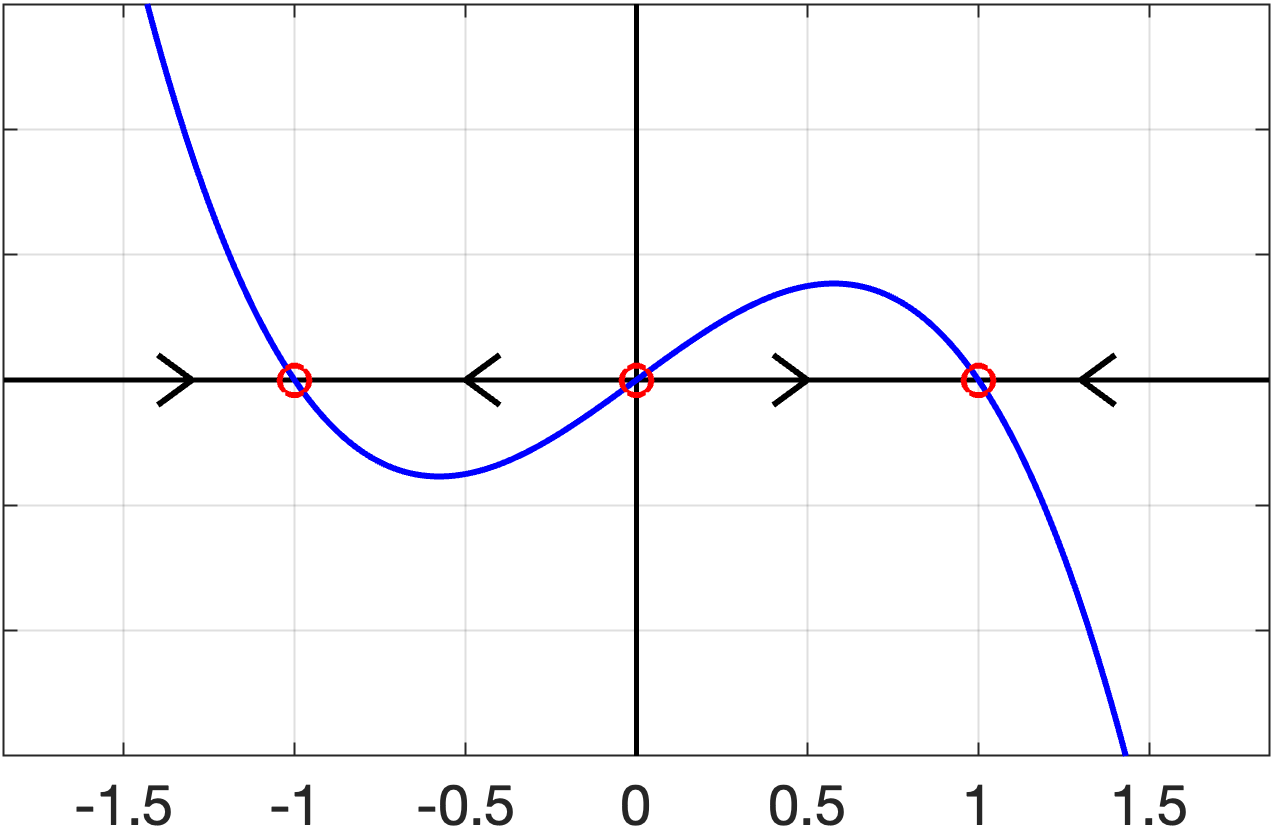
\includegraphics[width=.3\paperwidth]{media_paper/ACphase.png}
    \caption{The RHS of (\ref{eq_AC}) is plotted against $v$ when $v$ is $v$ is spatially constant. The phase plane shows that 1 and -1 are stable equilibria while 0 is unstable.}
    \label{fg_AC_phase}
\end{wrapfigure}
The Allen-Cahn equation (\ref{eq_AC}) admits three constant steady state solutions. These are obtained by solving the ODE 
\begin{equation} \label{eq_AC_ODE}
    0=\gamma\nabla^2v-\phi(v)
\end{equation}
when $\nabla v=0$. 
Note that (\ref{eq_AC_ODE}) is identical to the Euler Lagrange equation (\ref{eq_EL}) for the phase energy functional,
which implies that any stationary energy point is an equilibrium of (\ref{eq_AC}).
From (\ref{eq_AC_ODE}), we see that the constant equilibria are the zeros of $\phi$. 
The phase plane in Figure \ref{fg_AC_phase} shows the stability analysis. 
The solution $v=0$ is unstable, while $v=-1$ and $v=1$ are stable equilibria. 

\begin{wrapfigure}{r}{.4\paperwidth}
    \centering

    \vspace*{-19pt}
    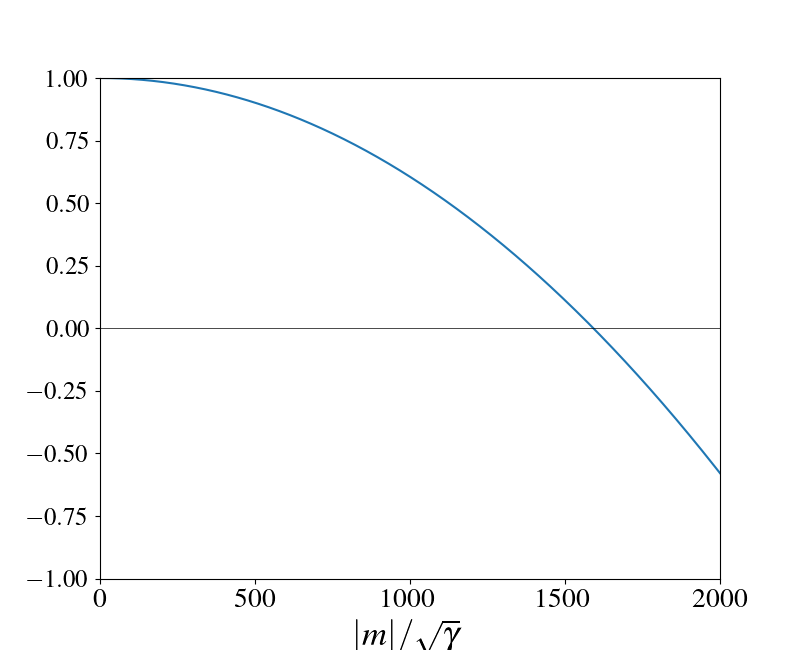
\includegraphics[width = .3\paperwidth]{media_paper/lin_AC_amp.png}

    \caption{The amplification factor of the solution to the Allen-Cahn equation linearized about 0 is plotted against $|k|/\sqrt{\gamma}$.}
    \vspace{-10pt}
    \label{fg_AC_amp_DE}
\end{wrapfigure}
The linearization of (\ref{eq_AC}) about the unstable equilibrium $v=0$ is 
\begin{equation} \label{eq_unstable_lin_AC}
    \frac{\partial v}{\partial t}=\gamma\nabla ^{2}v+v.
\end{equation}
For periodic boundary conditions, (\ref{eq_unstable_lin_AC}) has solution 
\begin{equation}
    v(x,t)=\sum_{m\in\mathbb{Z}^{d}}\widehat{[v_{0}]}_{m}~\e^{(1-4\pi^{2}\gamma|m|^{2})t}~\e^{2\pi\i m\cdot x},
\end{equation}
where the Fourier coefficients of the 1-periodic initial condition are given by 
\begin{equation} \label{eq_FC}
    \widehat{[v_{0}]}_{m}:=\int_{\Omega}v_{0}(x)~\e^{2\pi \i m\cdot x}~\ud x.
\end{equation}
The amplification factor is $1-4\pi^2\gamma|m|^2$ and is plotted in Figure \ref{fg_AC_amp_DE}. 
From the plot, we see that Fourier mode $m$ decays in time if $4\pi^{2}\gamma|m|^{2}>1$. This causes a low frequency instability. % FORMAT IS WEIRD
The constant mode will always be unstable. 
Whether additional modes are unstable depends on the value of $\gamma$. 
That a smaller value of $\gamma$ introduces higher frequency oscillations is consistent with its physical role in determining the width of phase boundaries. 
    
    
The linearized Allen-Cahn equation about the stable equilibrium $v=1$ is 
\begin{equation} \label{eq_lin_AC}
    \frac{\partial v}{\partial t}=\gamma\nabla ^{2}v+2-2v.
\end{equation}
For periodic boundary conditions, (\ref{eq_lin_AC}) has solution
\begin{equation} 
    v(x,t)=\sum_{m\in\mathbb{Z}^{d}}C_{m}~\e^{2\pi\i m\cdot x},
\end{equation}
where the constants $C_{m}$
\begin{equation}
    C_{m}:=\begin{cases}
    (\widehat{[v_{0}]}_{0}-1)\e^{-2t}+1 & m=0\\
    \widehat{[v_{0}]}_{m}~\e^{-[4\pi^{2}\gamma|m|^{2}+2]t} & m\ne0
    \end{cases}
\end{equation}
are related to the Fourier coefficients defined in (\ref{eq_FC}).
For the linear solution, the amplitudes of all non-constant Fourier modes decay exponentially in time. 
The constant mode approaches the steady state solution 1. 
The linearization about the other stable equilibrium similarly exhibits exponential decay of non-constant Fourier modes. 
However, the constant coefficient tends to -1.




\subsection{Finite Difference Approaches} \label{ssec_AC_FD}

We use the same discretization of the domains as in \ref{sssec_heat_fd} and analogously define 
\begin{align*}
	v_j^n&\approx v(jh,nk),\quad j\in[N]^d,n=0,1,\ldots\\
\end{align*}
The forward difference scheme (\ref{ds_HE_FD}) easily extends to the Allen-Cahn equation:
\begin{equation} \label{ds_AC_FD}
	\frac{v_j^{n+1}-v_j^n}{k}=\gamma\Delta v_j^n-\phi(v_j^n).{\tag{S3}}
\end{equation}
Due to the nonlinearity of $\phi$, a fully implicit scheme would require solving a nonlinear system of equations at each timestep. 
To improve numerical stability while still avoiding the associated computational costs, we use the semi-implicit method
\begin{equation} \label{ds_AC_CN}
    \frac{c_j^{n+1}-c_j^n}{k } =\gamma\Delta v_j^{n+1}-\phi(v_j^n). {\tag{S4}}
\end{equation}

The Fourier stability analysis performed in Section \ref{sssec_heat_fd} for the heat equation difference schemes relies on the linearity of the Fourier transform. 
Hence, it doesn't work for the nonlinear difference schemes (\ref{ds_AC_FD}) and (\ref{ds_AC_CN}). 
However, we can analyze the linearizations of (\ref{ds_AC_FD}) and (\ref{ds_AC_CN}) about the stable constant equilibria. 
We expect the stability of these linear schemes to reflect the stability of the nonlinear scheme, since solutions $v$ are bounded by -1 and 1. 
Linearizing the difference scheme (\ref{ds_AC_FD}) about the stable equilibrium $v=1$ gives
\begin{equation} \label{ds_lin_AC_FD}
    \frac{v_{j}^{n+1}-v_{j}^{n}}{k}=\Delta^{h}v_{j}^{n}+2-2v_{j}^{n}. \tag{lin-\ref{ds_AC_FD}}
\end{equation}
Write the solution $v_{j}^{n}$ as 
\begin{equation}
    v_{j}^{n}=\sum_{m\in [N]^{d}}\alpha_{m}^{n}~\e^{2\pi\i \frac{m\cdot j}{N}}
\end{equation}
using the DFT. In conjugate space, (\ref{ds_lin_AC_FD}) becomes 
\begin{equation} \label{eq_lin_AC_amps}
    \begin{cases}
        \alpha_{m}^{n+1}= \left(1- 2k\right)\alpha_{m}^{n}+ 2k & m=0\\
        \alpha_{m}^{n+1}= \left(1- 2k+k \gamma \lambda_{m}\right)\alpha_{m}^{n} & m\ne0.
    \end{cases}
\end{equation}
To satisfy the stability condition (\ref{eq_stab_cond}), we need the amplitudes of every Fourier mode to decay in time.
However, when $-1<\widehat{[v_{0}]}_{0}<1$ the no value of $k$ is sufficient.
In this case, $\alpha_{0}^{n}\to 1$ as $n \to \infty$. 
This is related to the Allen-Cahn equation failing to preserve mass in general.
Thus, we must use the modified stability condition
\begin{equation} 
    |\alpha_{m}^{n+1}|\le|\alpha_{m}^{n}|\quad \text{for all }m\ne0.
\end{equation}
From (\ref{eq_lin_AC_amps}), we have the amplification factor $1-2k+k\gamma\lambda_m$ for $m\ne0$.
Since the amplification factor is less than 1, stability follows from
\begin{equation} 
    1- 2k-4 \frac{k \gamma}{h^{2}}\sum_{i=1}^{d}\sin^{2}\left(\pi \frac{m_{i}}{J}\right)\ge-1.
\end{equation}
Using the a-priori bound $|\sin(x)|\le1$, 
\begin{equation} \label{eq_k_crit_AC}
    k_\text{crit}:=\frac{h^{2}}{h^{2}+2d\gamma}.
\end{equation}
Again, the analysis for the linearization of (\ref{ds_AC_FD}) about $v=-1$ reveals the same stability condition on $k$. 
Since $v=\pm1$ are stable equilibria of the Allen-Cahn equation and solutions are bounded between them, we expect the stability of the linearized scheme to at least determine an lower bound for the critical $k$ of the nonlinear scheme. 
Numerical experiments support this conclusion. Figure \ref{fg_nonlinear_stability_AC} shows a simulation which suggests the critical $k$ value for (\ref{ds_AC_FD}) is close to (\ref{eq_k_crit_AC}).

\def\ampwidth{.2\paperwidth}
\begin{figure}[H]
    \centering

    \begin{tabular}{ccc}
        $\gamma=.01h^2$ & $\gamma=1.00h^2$ & $\gamma=100.00h^2$ \\
        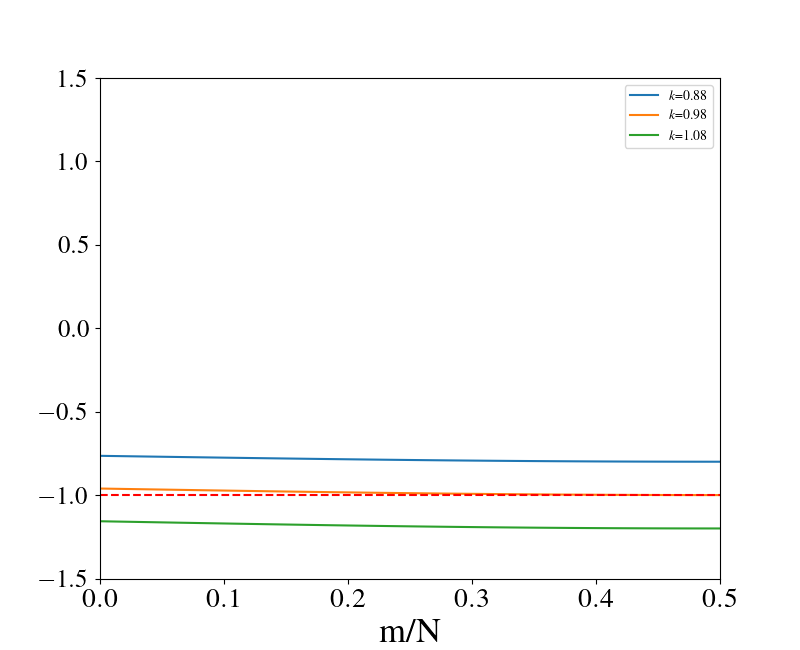
\includegraphics[width = \ampwidth]{media_paper/ga0.01_AC_FD.png} &
        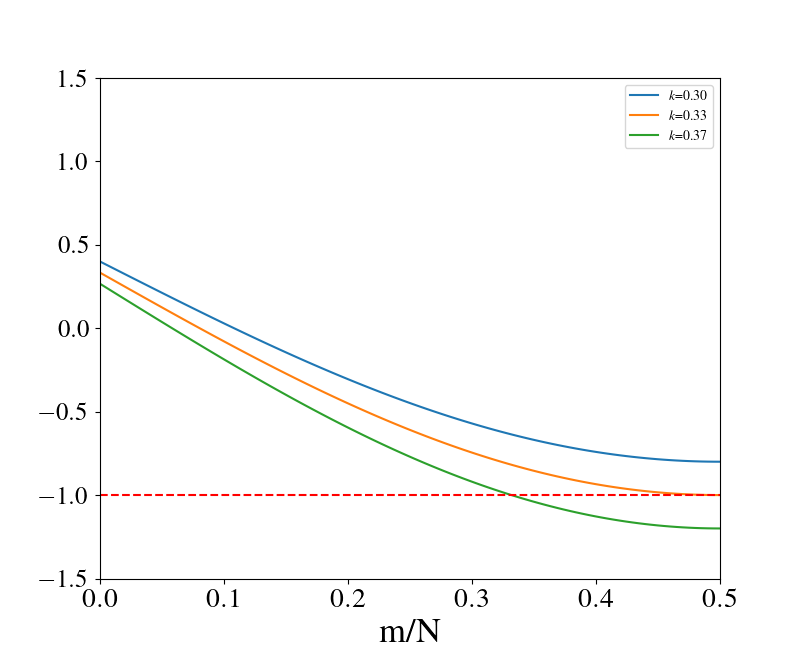
\includegraphics[width = \ampwidth]{media_paper/ga1_AC_FD.png} &
        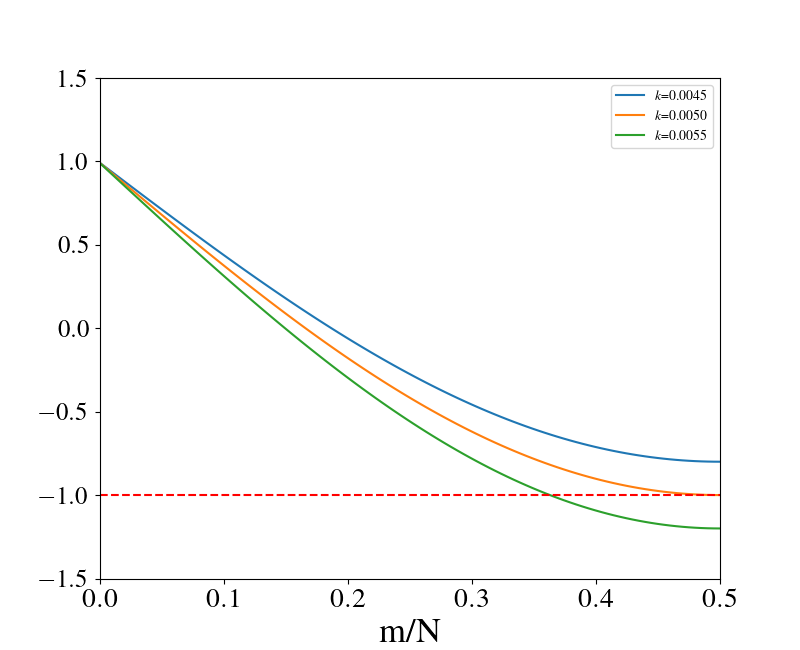
\includegraphics[width = \ampwidth]{media_paper/ga100_AC_FD.png}
    \end{tabular}

    \caption{The amplification factor for the linear difference scheme (\ref{ds_lin_AC_FD}) is plotted for different values of $\frac{k}{h^2}$ near $\frac{k_\text{crit}}{h^2}$. The left, middle and right plots have parameter values $\gamma=.01h^2$, $h^2$, and $100h^2$. When $k$ is above the critical value, the amplification factor dips below -1, showing a frequency instability for the difference scheme.}
    \label{fg_AC_amp}
\end{figure}
	
    
We can also perform this stability analysis on the linearization
\begin{equation}\label{ds_lin_AC_CN}
    \frac{v_{j}^{n+1}-v_{j}^{n}}{k}=\gamma \Delta^{h}v_{j}^{n+1}+2-2v_{j}^{n}\tag{lin-\ref{ds_AC_CN}}
\end{equation}
of the semi-implicit scheme (\ref{ds_AC_CN}).
The equivalent equation in Fourier space is
\begin{equation}
    \begin{cases}
        \alpha_{m}^{n+1}=\alpha_{m}^{n}+2k-2k \alpha_{m}^{n} & m=0 \\
        \alpha_{m}^{n+1}= \alpha_{m}^{n}+k \gamma \lambda_{m}\alpha_{m}^{n+1}-2k\alpha_{m}^{n} & m\ne0.
    \end{cases}
\end{equation}
For $m\ne0$, we have 
\begin{equation}
    (1-k \gamma \lambda_{m})\alpha_{m}^{n+1}=(1-2k)\alpha_{m}^{n},
\end{equation}
so amplitudes are decreasing in time if 
\begin{equation} 
    -1\le\frac{1-2k}{1-k \gamma \lambda_{m}}\le1.
\end{equation}
Since $\lambda_{m}\le0$, this holds whenever $1-2k>-1$. 
Thus, the stability condition for the semi-implicit linearized scheme (\ref{ds_lin_AC_CN}) is 
% \begin{equation}
    % k_\text{crit}= 1.
    $k_\text{crit}= 1.$
% \end{equation}
The superior stability of the nonlinear semi-implicit scheme is demonstrated in Figure (\ref{fg_nonlinear_stability_implicit_AC}).

\def\acfdwidth{.28\paperwidth}

\begin{figure}[H]
    \centering

    \begin{tabular}{cc}
        $k=k_\text{crit}$ & $k>k_\text{crit}$\\
        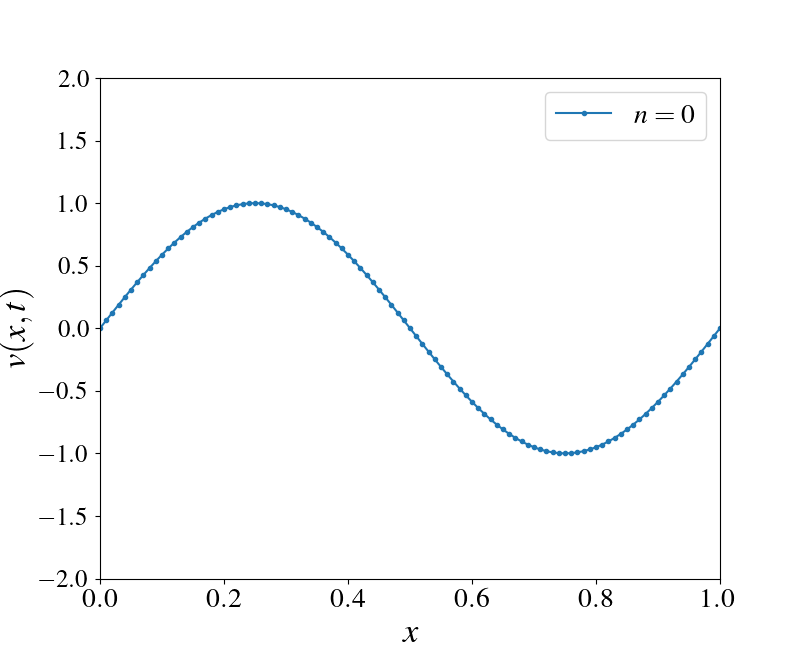
\includegraphics[width=\acfdwidth]{media_paper/stable_AC_FD_0} & 
        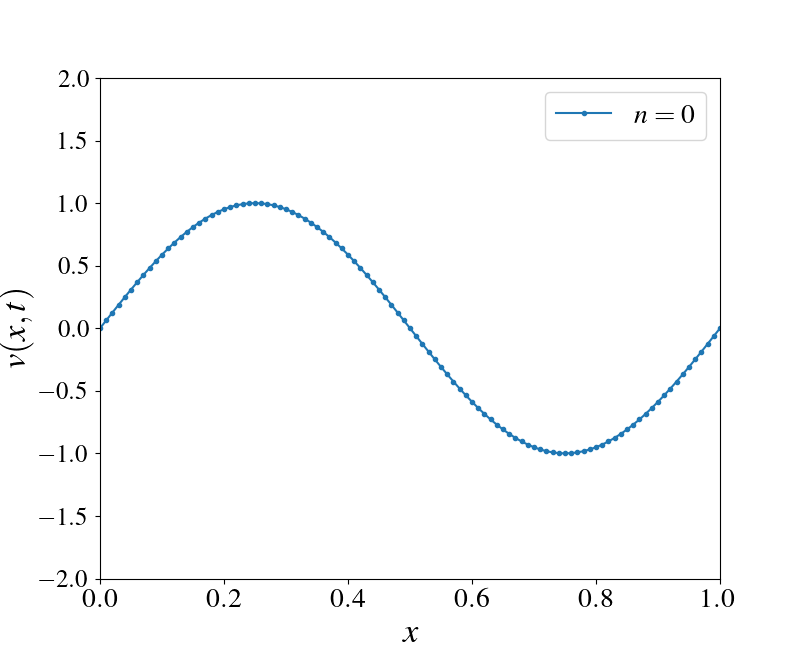
\includegraphics[width=\acfdwidth]{media_paper/unstable_AC_FD_0} \\
        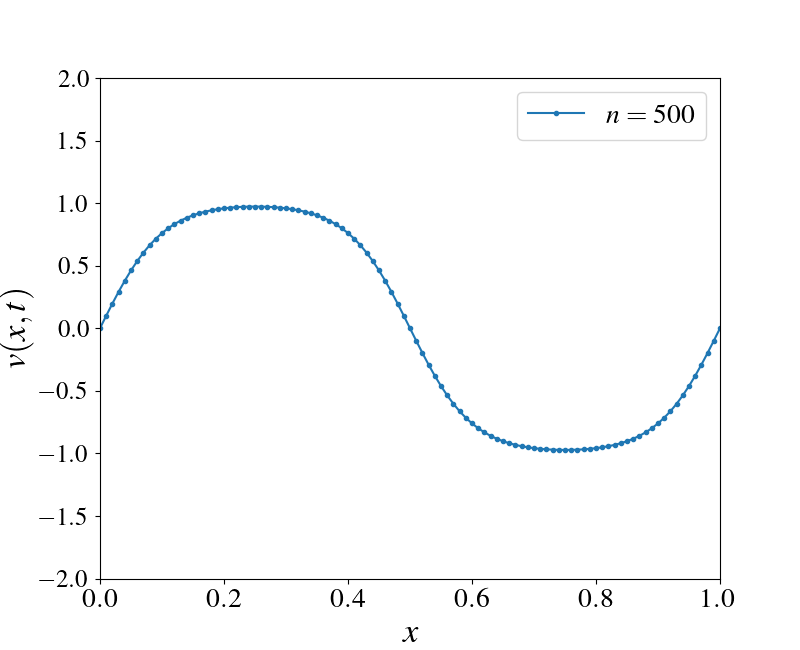
\includegraphics[width=\acfdwidth]{media_paper/stable_AC_FD_500} & 
        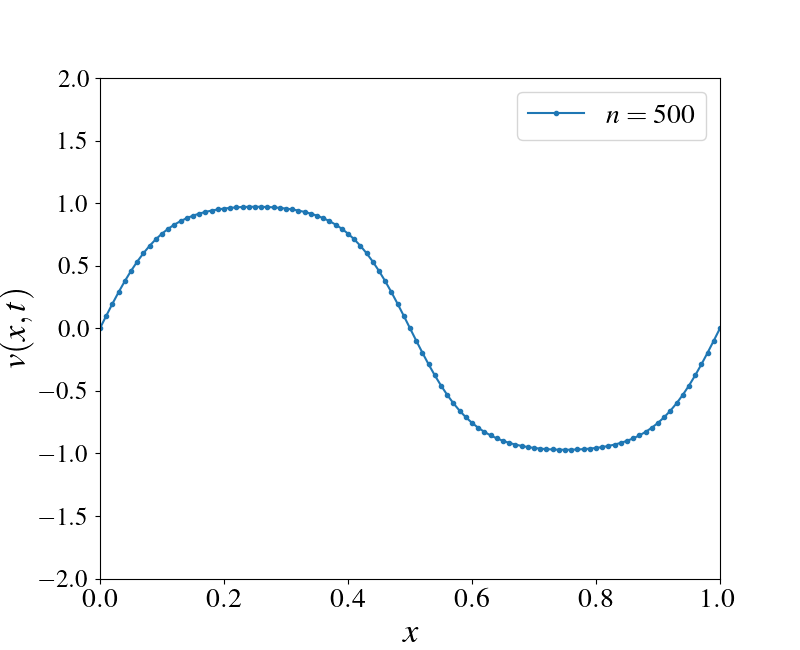
\includegraphics[width=\acfdwidth]{media_paper/unstable_AC_FD_500} \\
        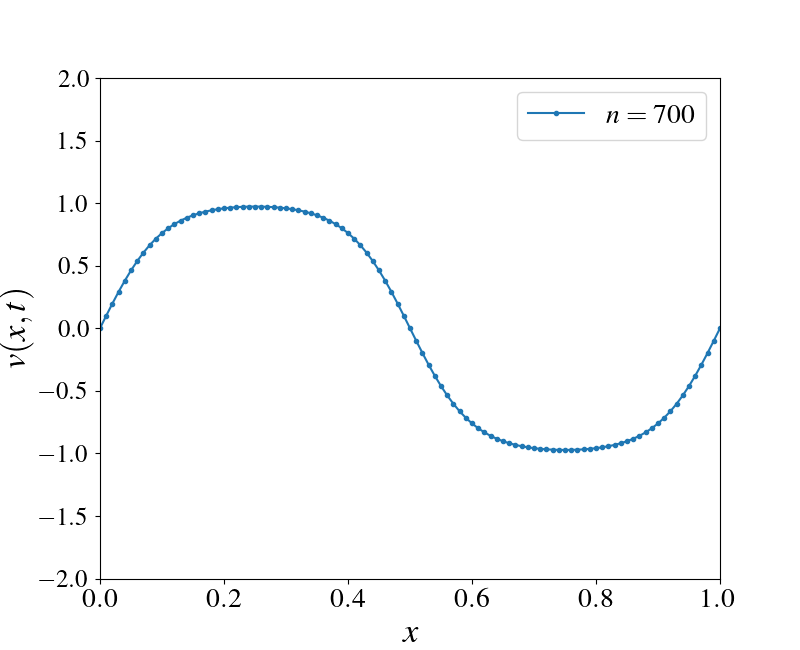
\includegraphics[width=\acfdwidth]{media_paper/stable_AC_FD_700} & 
        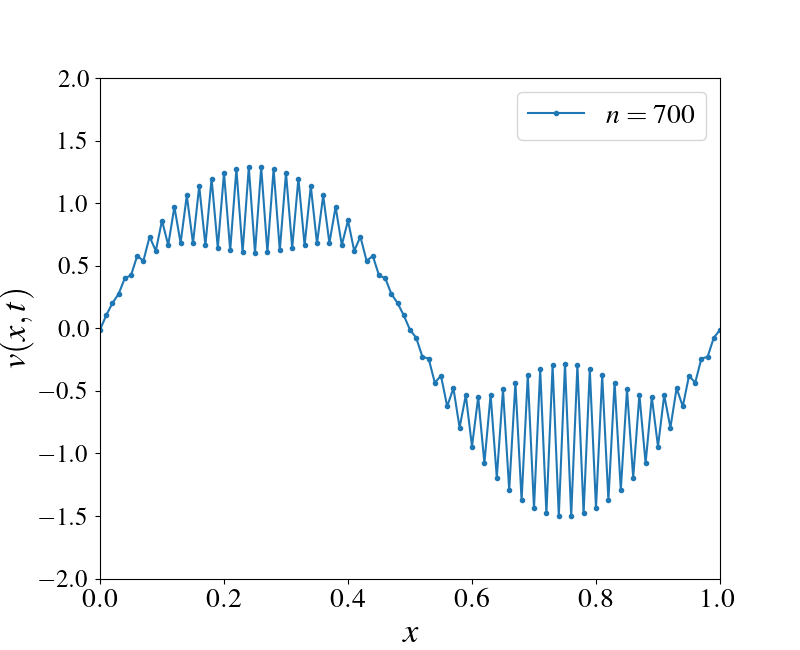
\includegraphics[width=\acfdwidth]{media_paper/unstable_AC_FD_700} \\
        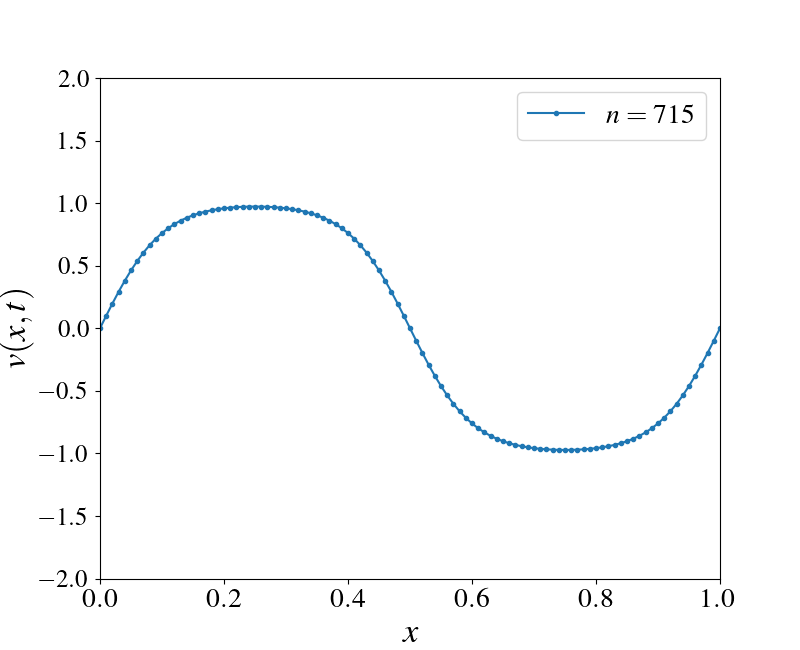
\includegraphics[width=\acfdwidth]{media_paper/stable_AC_FD_715} & 
        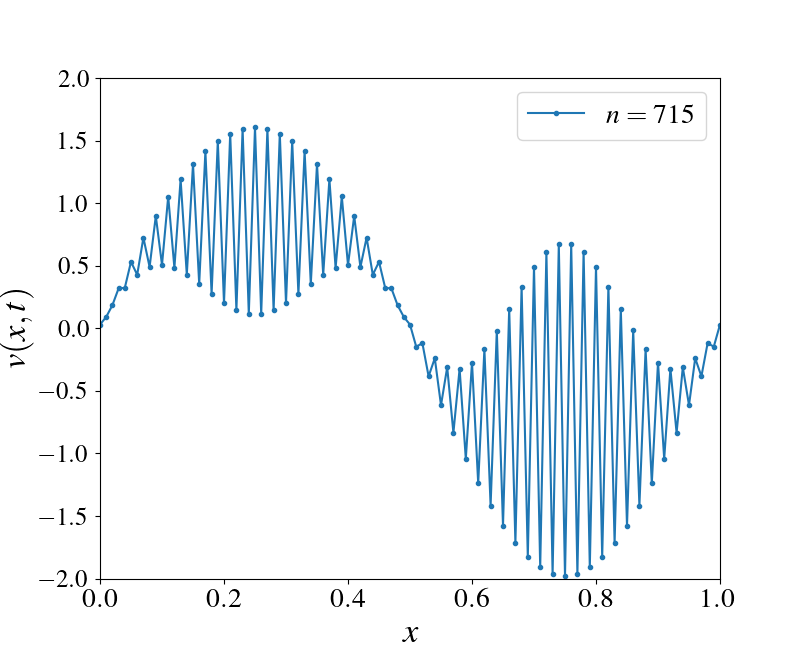
\includegraphics[width=\acfdwidth]{media_paper/unstable_AC_FD_715}
    \end{tabular}

    \caption{The nonlinear difference scheme (\ref{ds_AC_FD}) was solved in 1D for $h=.01,\gamma=.01$ from an initial state of a sine wave. On the left, $k=.0050=k_\text{crit}$ and on the right, $k=.0051>k_\text{crit}$, where $k_\text{crit}$ refers to the stability of the linear scheme (\ref{ds_lin_AC_FD}). When $k$ is greater than to the critical value of the linear scheme, the simulation displays numerical instability. However, $k=k_\text{crit}$ seems to be stable, suggesting that the stability condition for the linear scheme reflects the stability of the nonlinear scheme.}
    \label{fg_nonlinear_stability_AC}
\end{figure}

\begin{figure}[H]
    \centering

    \begin{tabular}{cc}
        $h=.01$ & $h=.005$ \\
        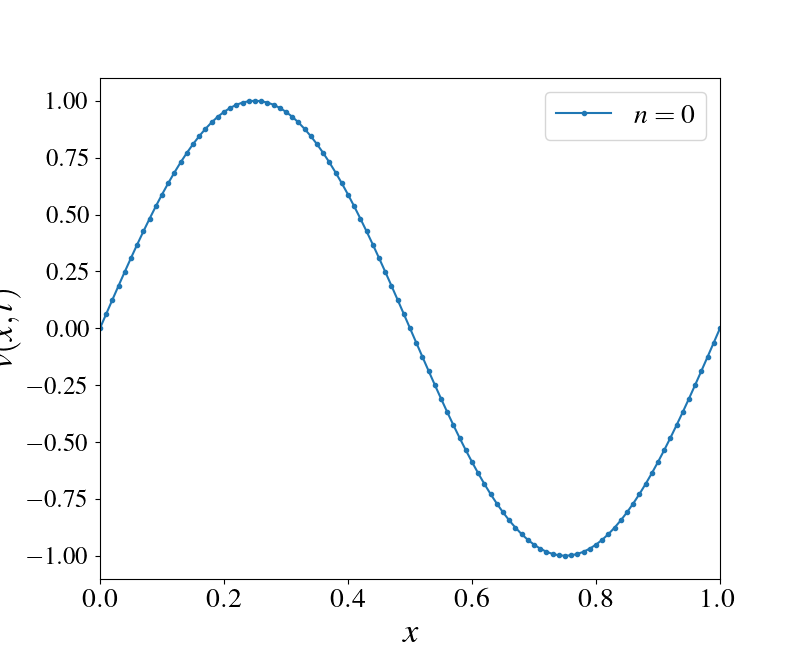
\includegraphics[width = \acfdwidth]{media_paper/stable_AC_CN_0} &
        \includegraphics[width = \acfdwidth]{media_paper/stable_AC_CN_0} \\
        \includegraphics[width = \acfdwidth]{media_paper/stable_AC_CN_1} &
        \includegraphics[width = \acfdwidth]{media_paper/stable_AC_CN_1} \\
        % \includegraphics[width = \acfdwidth]{media_paper/stable_AC_CN_2} &
        % \includegraphics[width = \acfdwidth]{media_paper/stable_AC_CN_2} \\
        \includegraphics[width = \acfdwidth]{media_paper/stable_AC_CN_5} &
        \includegraphics[width = \acfdwidth]{media_paper/stable_AC_CN_5} \\
        \includegraphics[width = \acfdwidth]{media_paper/stable_AC_CN_1000} &
        \includegraphics[width = \acfdwidth]{media_paper/stable_AC_CN_1000}
    \end{tabular}

    \caption{The nonlinear semi-implicit scheme was solved in 1D with different spatial resolutions $h=.01$ and $h=.005$ on the left and right. 
    Using the same initial condition and $\gamma$ as in Figure \ref{fg_nonlinear_stability_AC}, we see that the implicit scheme (\ref{ds_AC_CN}) has better stability properties than (\ref{ds_AC_FD}). 
    Additionally, its stability does not share the dependence on $h$.}
    \label{fg_nonlinear_stability_implicit_AC}
    
\end{figure}

\section{Cahn-Hilliard Equation} \label{sec_CH}

The full statement of the boundary value gradient flow of the phase energy functional over $H^{-1}_p$ is 
\begin{equation} \label{eq_CH}
    \left\{
        \begin{split}
            &\frac{\partial u}{\partial t}=M\nabla^2w&x\in\Omega,t>0\\
            &w=\phi(u)-\gamma\nabla^2u\\
            &u\big|_{x_i=0}=u\big|_{x_i=1},\quad w\big|_{x_i=0}=\mu\big|_{x_i=1}\quad&1\le i\le d\\
            &u_{x_i}\big|_{x_i=0}=u_{x_i}\big|_{x_i=1},\quad w_{x_i}\big|_{x_i=0}=\mu_{x_i}\big|_{x_i=1}\quad&1\le i\le d\\
            &u(x,0)=u_0(x)&x\in\Omega,
        \end{split}
    \right.
\end{equation}
where $\gamma$ is the phenomenological interfacial boundary parameter, $M$ is a mobility coefficient, $\phi=\psi'$ is the derivative of the free energy function, $\Omega=[0,1]^d$ is the spatial domain, and $c_0(x)$ is the initial condition \cite{copetti_1990_kinetics}. 



The periodic boundary conditions ensure that solutions $c$ to the Cahn-Hilliard equation (\ref{eq_CH}) satisfy the mass conservation constraint (\ref{eq_mass_con}). 
We apply (\ref{eq_CH}), the definition of the Laplacian operator, and linearity of the integral.
\begin{align}
    \frac{\ud}{\ud t}\int_{\Omega} c(x,t)~\ud x&=\int_{\Omega} \frac{\partial}{\partial t}c(x,t)~\ud x\label{eq_der_inside}\\
    &= M\int_{\Omega}\nabla^{2}w(x,t)\ud x\\
    &= M\int_{[0,1]^{d}}\sum_{n=1}^{d}\frac{\partial ^{2}w}{\partial x_{n}^{2}}(x,t)\ud x\\
    &= M\sum_{n=1}^{d}\int_{[0,1]^{d}}\frac{\partial ^{2}w}{\partial x_{n}^{2}}(x,t)\ud x\label{eq_end}.
\end{align}
In (\ref{eq_der_inside}), the Liebniz integration rule lets us move the time derivative inside the integral since $c$ is continuous in $x$. 
Without loss of generality, consider the first term of (\ref{eq_end}) and use the fundamental theorem of calculus to apply the boundary conditions
\begin{align}
    \int_{[0,1]^{d}}\frac{\partial ^{2}w}{\partial x_{1}^{2}}\ud x_{1}\cdots \ud x_{d}&= \int_{[0,1]^{d-1}} \frac{\partial w}{\partial x_{1}}(x_{1},\dots,t)\bigg|_{x_{1}=0}^{1}\ud x_{2}\cdots \ud x_{d}\\
    &= \int_{[0,1]^{d-1}}\frac{\partial w}{\partial x_{1}}(1,\ldots,t)-\frac{\partial w}{\partial x_{1}}(0,\ldots,t)\ud x_{2}\cdots\ud x_{d}\\
    &= 0.
\end{align}
Thus, each term of the sum (\ref{eq_end}) is 0, and mass is constant in time. 


\subsection{Linear Stability Analysis}

Like for the Allen-Cahn equation, any equilibrium solution to the Cahn-Hilliard equation satisfies the Euler-Lagrange equation (\ref{eq_EL}) for the phase energy functional \cite{novickcohen_1984_nonlinear}.
\begin{wrapfigure}{r}{.4\paperwidth}
    \centering

    \includegraphics[width = .4\paperwidth]{media_paper/lin_CH_amp.png}

    \caption{The amplification factor $-A_{|m|}$ for solutions to the Cahn-Hilliard equation linearized about $c_0$ is plotted against wavenumber. 
    When $c_0$ is in the spinodal region, the linear solutions display a low-frequency instability for all wavenumbers $m$ with $|m|<m_c$.
    The fastest growing wavenumbers have $|m|=m_m\in(0,m_c)$. \cite{copetti_1990_kinetics}}
    \label{fg_unstable_lin_CH}
\end{wrapfigure}
Any constant function $c=c_0$ is an equilibrium solution of the Cahn-Hilliard equation (\ref{eq_CH}).
Linearizing about $c_0$ gives
\begin{equation} \label{eq_lin_CH}
    \frac{\partial c}{\partial t}=M[\phi'(c_{0})\nabla ^{2}c-\gamma \nabla ^{2}(\nabla ^{2}c)].
\end{equation}
For periodic boundary conditions (\ref{eq_lin_CH}) has solution 
\begin{align}
    c(x,t)&=\sum_{m\in\mathbb{Z}^{d}}\widehat{[c_0]}_m~\e^{-A_{|m|t}}~\e^{2\pi\i m\cdot x}\\
    A_{|m|}&=-4\pi^2M|m|^2[\phi'(c_0)+4\pi^2\gamma|m|^2]
    % c(x,t)=\sum_{m\in\mathbb{Z}^{d}}\widehat{[c_{0}]}_{m}~\e^{4 \pi^{2}M|m|^{2}[\phi'(c_{0})+4\pi^{2}\gamma|m|^{2}]t}~\e^{2\pi\i m\cdot x}
    .
\end{align}
When $\phi'(c_{0})>=0$, $A_{|m|}>0$ for all $m$. 
So, every non-constant Fourier mode except $m=0$ decays in time, causing solutions to the linear equation to converge to their constant average. 
When $\phi'(c_{0})<0$, $c_{0}$ is in the unstable region. 
Just as with the linearization of the Allen-Cahn equation about its unstable constant equilibrium, there is a low frequency instability. 
Again, the number of modes which grow in time depends on the parameter $\gamma$. 
Here, the fastest growing mode is not be the constant mode, as shown by thr amplification factor plot in Figure \ref{fg_unstable_lin_CH}. 





\subsection{Finite Difference Approaches} \label{sssec_CH_FD}

We use the same discretization of the domains as in \ref{sssec_heat_fd} and analogously define 
\begin{align*}
	c_j^n&\approx c(jh,nk),\quad j\in[N]^d,n=0,1,\ldots\\
	% w_j^n&\approx w(jh,nk),\quad j\in\{0,\ldots,J\}^d,n=0,\ldots,N
\end{align*}
The forward difference scheme (\ref{ds_HE_FD}) easily extends to the Cahn-Hilliard equation: 
\begin{equation} \label{ds_CH_FD}
	% \frac{c_j^{n+1}-c_j^n}{k}=M\Delta^hw_j^n= M\Delta^h(\phi(c_j^n))-M\gamma\Delta^h(\Delta^h c_j^n){\tag{S5}}
	\frac{c_j^{n+1}-c_j^n}{k}=M\Delta^h(\phi(c_j^n))-M\gamma\Delta^h(\Delta^h c_j^n).{\tag{S5}}
\end{equation}
Again, we use a semi-implicit scheme
\begin{equation} \label{ds_CH_CN}
    \frac{c_j^{n+1}-c_j^n}{k } =M\Delta^h(\phi(c_j^n))-M\gamma\Delta^h(\Delta^hc_j^{n+1}){\tag{S6}}
\end{equation}
to avoid solving a nonlinear system at each timestep. 

Just as with the difference schemes from the heat equation, the discrete mass conservation condition (\ref{eq_discrete_con}) extends from the differential equation to the difference schemes.
Writing 
\begin{align*}
	c_j^n&=\sum_{m\in[N]^d}\alpha_m^n~\e^{2\pi\i\frac{m\cdot j}{J}}\\
	% w_j^n&=\sum_m\beta^n~\e^{2\pi\i\frac{m\cdot j}{J}}\\
    \phi(c_j^n)-\gamma\Delta^hc_j^n&=\sum_{m\in[N]^d}\beta_m^n~\e^{2\pi\i\frac{m\cdot j}{N}}\\
    \phi(c_j^n)-\gamma\Delta^hc_j^{n+1}&=\sum_{m\in[N]^d}\delta_m^n~\e^{2\pi\i\frac{m\cdot j}{N}},
\end{align*}
we see
\begin{equation*}
	\alpha_0^{n+1}=\alpha_0^n+\lambda_0\beta_0^n=\alpha_0^n
\end{equation*}
for (\ref{ds_CH_FD}), and 
\begin{equation*}
    \alpha_0^{n+1}=\alpha_0^n+\lambda_0\delta_0^n=\alpha_0^n
\end{equation*}
for (\ref{ds_CH_CN}).


As with the Allen-Cahn equation, the nonlinearity of the difference schemes for the Cahn-Hilliard equation prevent a direct Fourier analysis from determining their stability.
However, we can linearize the difference scheme (\ref{ds_CH_FD}) about a stable constant equilibrium $c=c_{0}$, $|c_{0}|\ge \frac{1}{\sqrt{3}}$, giving 
\begin{equation} \label{ds_lin_CH_FD}
\frac{c_{j}^{n+1}-c_{j}^{n}}{k}=M\phi'(c_{0})\Delta^{h}c_{j}^{n}-M\gamma \Delta^{h}(\Delta^{h}c_{j}^{n}). \tag{lin-S5}
\end{equation}
Using the standard DFT representation of $c_{j}^{n}$, this gives the equation 
\begin{equation} 
    \alpha_{m}^{n+1}=\alpha_{m}^{n}+kM\phi'(c_{0})\lambda_{m}\alpha_{m}^{n}-kM\gamma \lambda_{m}^{2}\alpha_{m}^{n}=(1+kM\phi'(c_{0})\lambda_{m}-kM\gamma\lambda_{m}^{2})\alpha_{m}^{n}
\end{equation}
in conjugate space.
We have the amplification factor $1+kM\phi'(c_0)\lambda_m-kM\gamma\lambda^2_m$, which is plotted in Figure \ref{fg_CH_amp_FD}
Since we are considering a stable equilibrium $c_{0}$, $\phi'(c_{0})\ge0$. 
Therefore, the stability condition (\ref{eq_stab_cond}) becomes 
\begin{equation} 
    |1+\underbrace{kM\phi'(c_{0})\lambda_{m}-kM\gamma \lambda_{m}^{2}}_{\le0}|\le1\iff1+kM\phi'(c_{0}\lambda_{m}-kM\gamma \lambda_{m}^{2})\ge-1.
\end{equation}
This holds generally if 
\begin{equation} 
    k\le k_\text{crit}= \frac{h^{4}}{M[8d\gamma+2d^{2}h^{2}\phi'(c_{0})]}.
\end{equation}
For the extreme equilibria $c=1$ and $c=-1$, we have a minimal value of $k_\text{crit}$ at 
\begin{equation} \label{eq_CH_FD_stab}
k'_\text{crit}= \frac{h^{4}}{M[8d\gamma+4d^{2}h^{2}]}.
\end{equation}
Figure \ref{fg_nonlinear_stability_CH} supports the use of (\ref{eq_CH_FD_stab}) as an estimate of the stability of the nonlinear difference scheme (\ref{ds_CH_FD}).
Note that the mass-conservation of the Cahn-Hilliard difference schemes allowed us to use the standard stability condition (\ref{eq_stab_cond}).

\begin{figure}[H] 
    \centering
    
    \begin{tabular}{ccc}
        $\gamma=.01h^2$ & $\gamma=1.00h^2$ & $\gamma=100.00h^2$ \\
        \includegraphics[width = \ampwidth]{media_paper/ga0.01_CH_FD.png} &
        \includegraphics[width = \ampwidth]{media_paper/ga1_CH_FD.png} &
        \includegraphics[width = \ampwidth]{media_paper/ga100_CH_FD.png}
    \end{tabular}

    \caption{The amplification factor for the linear difference scheme (\ref{ds_lin_CH_FD}) is plotted for different values of $\frac{kM}{h^2}$ near $\frac{k_\text{crit}M}{h^2}$. The left, middle and right plots have parameter values $\gamma=.01h^2$, $h^2$, and $100h^2$. When $k$ is above the critical value, the amplification factor dips below -1, showing a frequency instability for the difference scheme. For simplicity, $M=1$.}
    \label{fg_CH_amp_FD}
\end{figure}



Linearizing the semi-implicit difference scheme (\ref{ds_CH_CN}) about a stable constant equilibrium $c=c_{0}$ gives
\begin{equation} \label{ds_lin_CH_CN}
    \frac{c_{j}^{n+1}-c_{j}^{n}}{k}=M\phi'(c_{0})\Delta^{h}u_{j}^{n}-M\gamma \Delta^{h}(\Delta^{h}u_{j}^{n+1}). \tag{lin-S6}
\end{equation}
In Fourier space, we have the equation 
\begin{equation}
    \alpha_{m}^{n+1}=\alpha_{m}^{n}+kM\phi'(c_{0})\lambda_{m}\alpha_{m}^{n}-Mk \gamma \lambda_{m}^{2}\alpha_{m}^{n+1}.
\end{equation}
The amplification factor is given below and plotted in Figure \ref{fg_CH_amp_CN}. 
\begin{equation}  \label{eq_small_ga}
    \left| \frac{\alpha_{m}^{n+1}}{\alpha_{m}^{n}}\right|=\left| \frac{1+kM\phi'(c_{0})\lambda_{m}}{1+kM\gamma \lambda_{m}^{2}}\right|\le|1+kM\phi'(c_{0})\lambda_{m}|
\end{equation}
which is a good approximation for small $\gamma$. 
Since $c_{0}$ is a stable equilibrium, we have $\phi'(c_{0})\lambda_{m}\le0$, which gives the stability condition 
\begin{equation} 
    k\le - \frac{2}{M\phi'(c_{0})\lambda_{m}}\le \frac{h^{2}}{2dM\phi'(c_{0})}.
\end{equation}
At the extreme equilibria $c_{0}=\pm1$, we have 
\begin{equation} 
    k_\text{crit}= \frac{h^{2}}{4dM}.
\end{equation}
It is not surprising that this semi-implicit scheme has stability $O(h^{2})$ while the other (semi)-implicit linear schemes (\ref{ds_HE_CN}) and (\ref{ds_lin_AC_CN}) are $O(1)$ in $h$ since we handled the derivative of the approximation of the nonlinear term explicitly.
This should align with the nonlinear difference scheme where explicit treatment of the nonlinear term is essential to avoid solving a nonlinear system at each step. 
Figure \ref{fg_nonlinear_stability_implicit_CH} suggests that $k_\text{crit}$ is a good approximation of the stability of the nonlinear scheme (\ref{ds_CH_CN}) when $\gamma$ is small.
When the approximation in (\ref{eq_small_ga}) does not hold, $k_\text{crit}$ is at least a lower bound.

\begin{figure}[H]
    \centering
    
    \begin{tabular}{ccc}
        $\gamma=.01h^2$ & $\gamma=1.00h^2$ & $\gamma=100.00h^2$ \\
        \includegraphics[width = \ampwidth]{media_paper/ga0.01_CH_CN.png} &
        \includegraphics[width = \ampwidth]{media_paper/ga1_CH_CN.png} &
        \includegraphics[width = \ampwidth]{media_paper/ga100_CH_CN.png}
    \end{tabular}

    \caption{The amplification factor for the linear difference scheme (\ref{ds_lin_CH_CN}) is plotted for different values of $\frac{kM}{h^2}$ near $\frac{k_\text{crit}M}{h^2}$.  The left, middle and right plots have parameter values $\gamma=.01h^2$, $h^2$, and $100h^2$. When $k$ is above the critical value and the small $\gamma$ approximation holds, the amplification factor dips below -1, showing a high frequency instability for the difference scheme. For simplicity, $M=1$.}
    \label{fg_CH_amp_CN}
\end{figure}

\begin{figure}[H] 
    \centering

    \begin{tabular}{cc}
        $k=k_\text{crit}$ & $k>k_\text{crit}$ \\
        \includegraphics[width = \acfdwidth]{media_paper/stable_CH_FD_0} & 
        \includegraphics[width = \acfdwidth]{media_paper/unstable_CH_FD_0} \\
        % \includegraphics[width = \acfdwidth]{media_paper/stable_CH_FD_400} & 
        % \includegraphics[width = \acfdwidth]{media_paper/unstable_CH_FD_400} \\
        \includegraphics[width = \acfdwidth]{media_paper/stable_CH_FD_1000} & 
        \includegraphics[width = \acfdwidth]{media_paper/unstable_CH_FD_1000} \\
        \includegraphics[width = \acfdwidth]{media_paper/stable_CH_FD_2600} & 
        \includegraphics[width = \acfdwidth]{media_paper/unstable_CH_FD_2600} \\
        \includegraphics[width = \acfdwidth]{media_paper/stable_CH_FD_2770} & 
        \includegraphics[width = \acfdwidth]{media_paper/unstable_CH_FD_2770} \\
        % \includegraphics[width = \acfdwidth]{media_paper/stable_CH_FD_5000} & 
        % \includegraphics[width = \acfdwidth]{media_paper/unstable_CH_FD_5000} \\
    \end{tabular}

    \caption{The nonlinear difference scheme (\ref{ds_CH_FD}) was solved for $h=.01,\gamma=.001,M=1$ from an initial state of a sine wave. 
    On the left, $k=.00000120=k_\text{crit}$ and on the right, $k=.00000122>k_\text{crit}$, where $k_\text{crit}$ refers to the stability of the linear scheme (\ref{ds_lin_CH_FD}). 
    When $k$ is greater than the critical value of the linear scheme, the simulation displays numerical instability. 
    However, $k=k_\text{crit}$ seems to be stable up to $n=10000$, suggesting that the stability condition for the linear scheme reflects the stability of the nonlinear scheme.}

    \label{fg_nonlinear_stability_CH}
\end{figure}

    
\begin{figure}[H]

    \def\acfdwidth{.25\paperwidth}

    \centering
    
    \begin{tabular}{ccc}
        $k=.1k_\text{crit}$ & $k=k_\text{crit}$ & $k>k_\text{crit}$ \\
        \includegraphics[width = \acfdwidth]{media_paper/very_stable_CH_CN_0.png} &
        \includegraphics[width = \acfdwidth]{media_paper/stable_CH_CN_0} &
        \includegraphics[width = \acfdwidth]{media_paper/unstable_CH_CN_0} \\
        % \includegraphics[width = \acfdwidth]{media_paper/very_stable_CH_CN_10.png} &
        % \includegraphics[width = \acfdwidth]{media_paper/stable_CH_CN_1} &
        % \includegraphics[width = \acfdwidth]{media_paper/unstable_CH_CN_1} \\
        % \includegraphics[width = \acfdwidth]{media_paper/very_stable_CH_CN_100.png} &
        % \includegraphics[width = \acfdwidth]{media_paper/stable_CH_CN_10} &
        % \includegraphics[width = \acfdwidth]{media_paper/unstable_CH_CN_10} \\
        \includegraphics[width = \acfdwidth]{media_paper/very_stable_CH_CN_1000.png} &
        \includegraphics[width = \acfdwidth]{media_paper/stable_CH_CN_100} &
        \includegraphics[width = \acfdwidth]{media_paper/unstable_CH_CN_100} \\
        % \includegraphics[width = \acfdwidth]{media_paper/very_stable_CH_CN_10000.png} &
        % \includegraphics[width = \acfdwidth]{media_paper/stable_CH_CN_1000} &
        % \includegraphics[width = \acfdwidth]{media_paper/unstable_CH_CN_1000} \\
        \includegraphics[width = \acfdwidth]{media_paper/very_stable_CH_CN_32000.png} &
        \includegraphics[width = \acfdwidth]{media_paper/stable_CH_CN_3200} &
        \includegraphics[width = \acfdwidth]{media_paper/unstable_CH_CN_3200} \\
        \includegraphics[width = \acfdwidth]{media_paper/very_stable_CH_CN_32170.png} &
        \includegraphics[width = \acfdwidth]{media_paper/stable_CH_CN_3217} &
        \includegraphics[width = \acfdwidth]{media_paper/unstable_CH_CN_3217} \\
        % \includegraphics[width = \acfdwidth]{media_paper/very_stable_CH_CN_50000.png} \\
        % \includegraphics[width = \acfdwidth]{media_paper/stable_CH_CN_5000} &
        % \includegraphics[width = \acfdwidth]{media_paper/unstable_CH_CN_5000} \\
    \end{tabular}

    \caption{
        The nonlinear difference scheme (\ref{ds_CH_CN}) was solved for $h=.01,\gamma=1e-6,M=1$ from an initial state of a sine wave. 
        On the left, $k=.0000025=.1k_\text{crit}$, in the middle, $k=.000025=k_\text{crit}$, and on the right, $k=.000026>k_\text{crit}$, where $k_\text{crit}$ refers to the stability of the linear scheme (\ref{ds_lin_CH_CN}). 
        When $k$ is greater than to the critical value of the linear scheme, the simulation displays numerical instability. 
        However, $k=k_\text{crit}$ seems to be stable up to $n=10000$, suggesting that the stability condition for the linear scheme reflects the stability of the nonlinear scheme.
        While it may look like each scheme is unstable in interface region from $n=100$ on, this is actually a phase separation effect.
        That the schemes for $k=k_\text{crit}$ and $k=.1k_\text{crit}$ are the same supports this conclusion.
        The reason for separation on the grid precision is the small value of $\gamma$, which was chosen to make the stability estimate hold.
    }
    \label{fg_nonlinear_stability_implicit_CH}
\end{figure}



\section{Phase Separation Molecular Dynamics} \label{ssec_phase_MD}

As in diffusion, we use the Leonard-Jones model for interparticle interactions. 
We have the same interparticle potential
\begin{equation}
    V_{ij}=4\epsilon_{ij}\left[ \left( \frac{\sigma_{ij}}{r_{ij}} \right)^{12}-\left( \frac{\sigma_{ij}}{r_{ij}} \right)^6 \right].
\end{equation}

\begin{wraptable}{r}{.3\paperwidth}
    
    \centering
    \begin{tabular}{|l|l|l|}
        \hline
        Interaction & $\epsilon$ & $\sigma$ \\
        \hline
        $A-A$ & 3.0 & 1.0 \\
        \hline
        $B-B$ & 3.0 & 1.0 \\
        \hline
        $A-B$ & 1.0 & 1.0 \\
        \hline
    \end{tabular}

    \caption{Leonard-Jones parameter values for phase separation MD simulation.}
    \label{tb_lj_phase}
\end{wraptable}
For our two-component system, we denote atom types as $A$ and $B$. 
The interactions between particles of the same type are determined by $\epsilon_{AA},\sigma_{AA}$ and $\epsilon_{BB },\sigma_{BB}$. 
For cross interactions, we have $\epsilon_{AB }$ and $\sigma_{AB}$. 
Taking 
\begin{equation} \label{eq_phase_req}
    \epsilon_{AA}\sim\epsilon_{BB}<<\epsilon_{AB},\quad \sigma_{AA}\sim\sigma_{BB}\sim\sigma_{AB}
\end{equation}
makes interactions between like particles stronger than opposite particles. 
With a sufficiently high pressure, this causes $A$ and $B$ to separate into pure regions.
Choosing $\epsilon_{AA}=\epsilon_{BB}$ is consistent with choosing the free energy function $\psi$ in the differential equation models to be symmetric.
For our MD simulation, we used the parameter values in Table \ref{tb_lj_phase}, which are consistent with (\ref{eq_phase_req}).


\subsection{Parameter Estimation} \label{ssec_phase_estim}


Estimating the order parameter of the MD simulation has an additional step for the two component system.
We first approximate the mole fractions of each component $A_j^n$ and $B_j^n$ on a grid with the binning procedure
\begin{equation}
    A_j^n=\frac{\#\{A\text{ atoms in bin }j\}}{\#\left\{  \text{atoms in bin }j\right\}}.
\end{equation}
Then, the order parameter is the difference between the concentrations:
\begin{equation}
    U_j^n=A_j^n-B_j^n.
\end{equation}

We can extend the parameter estimation procedure from Section {\ref{ssec_diff_estim}} to the Allen-Cahn and Cahn-Hilliard models.
For consistency, we added the mobility coefficient to the Allen-Cahn equation, so the two models are
\begin{align}
    \frac{\partial v}{\partial t}&=M[\gamma\nabla^2v-\phi(v)]\tag{AC}\\
    \frac{\partial c }{\partial t }&=M\nabla^2[\phi(v)-\gamma\nabla^2c]\tag{CH}
\end{align}
with appropriate periodic boundary conditions.
The main difference from the previous estimation procedure is the second parameter $\gamma$.
Nevertheless, our previous implementation was able to handle arbitrarily many parameters, so this is not an issue.


\section{Results}

We will show results for two-dimensional simulations of molecular dynamics and continuum phase separation, although the algorithms are easily extended to three dimensions.
We impose periodicity on the MD domain boundary, matching the differential equation boundary conditions.
We conducted a LAMMPS simulation of a two-component Leonard-Jones fluid phase separating.
Selected snapshots of the MD trajectory are shown in Figure \ref{fg_AC_phase}.

We used the Leonard-Jones unit system of LAMMPS \cite{LAMMPS}. 
All units are based on a distance of $\sigma$, an energy of $\epsilon$, and a mass $m$.
The values of the Leonard-Jones parameters are shown in Table \ref{tb_lj_phase}.
Unlike for diffusion, we manually set the mixed interaction term to facilitate phase separation.
We set the mass of each particle to 1.
The MD simulation box was 300 $\times$ 300.
There were 35000 $A$ atoms and 35000 $B$ atoms.
The simulation proceeds from a pseudo-random initial condition. 
The densities and order parameter for the initial condition are given by
\begin{equation} \label{eq_phase_IC}
\begin{split}
    x_A(x,y)&=(1+.5\sin(2\pi x))(1+.5\sin(2\pi y))\\
    x_B(x,y)&=(1-.5\sin(2\pi x))(1-.5\sin(2\pi y))\\
    v(x,y)&=x_A(x,y)-x_B(x,y)=.5\sin(2\pi x)+.5\sin(2\pi y) .
\end{split}
\end{equation}
The particles were imbued with initial velocities satisfying the Maxwell-Boltzmann distribution of velocities for $T=1$. 
The temperature and pressure stabilized around 1.3 and 1.8, respectively.
The critical cutoff for interparticle interactions was $r_c=2.5$.
The timestep was $k_\text{md}=.01$ and the MD simulation was run for 4e6 timesteps.

From the simulation, we use the procedure outlined in Section \ref{ssec_phase_estim} to estimate the differential equation parameters $M$ and $\gamma$.
To reduce computational complexity, we use a larger timestep $k=4000k_{\text{md}}$ for the difference equation model and only consider every 4000 MD timesteps. 
This gives $n_\text{max}=1000$. The estimation procedure generates an estimates $\hat M_N$ and $\hat \gamma_N$ for each binning precision N = 20, 50, 100. 
The result of solving the Allen-Cahn and Cahn-Hilliard equations for their respective $\hat M_{50}$ and $\hat \gamma_{50}$ and spatial resolution $N = 50$ is shown alongside the estimated order parameter with binning precision of 50 in Figure \ref{fg_phase_results}.
Table \ref{tb_phase_data} shows the error of solving each differential equation using the pair of estimated parameters at the different spatial resolutions.

We note one distinction between the Allen-Cahn and Cahn-Hilliard models that shows up in the data.
At the final timestep, we see phase separation in both systems.
However, the regions where the initial order parameter was 0 between two like phases behave differently.
In the Allen-Cahn equation, we see the red regions have combined in both the top right and bottom left corner.
However, in the Cahn-Hilliard model, they have combined in the bottom left and separated in the top right.
We attribute this difference to the fact that the Cahn-Hilliard equation preserves mass, while the Allen-Cahn equation does not.
In both models, which place and which phase they selected came from the randomness of the initial condition.
However, the Cahn-Hilliard solution had to have the red phases combine in one corner and the blue combine in the other.

The future research directions mentioned in Section \ref{sec_diff_res} also apply here. 
Additionally, several questions unique to the phase separation problem should be addressed.

\begin{itemize}

\item In the final timestep MD snapshot of Figure \ref{fg_phase_results} we notice patches of $B$ particles in the large regions of $A$ and vice versa.
These are not present in the solution to either differential equation.
Qualitatively, this is the main difference between the MD and continuum results.
There are a couple possible explanations for this difference.
One is that the parameter estimation failed to equate the timescales. 
The MD simulation is yet to reach its equilibrium where these small patches will disappear, as they have in the equilibrium of the differential equations.
Conducting longer and larger MD simulations could confirm whether equilibrium has been reached.
Alternatively, this aspect of phase separation dynamics may be beyond what the continuum model can capture.


\item It would be interesting to look at cost metrics other than direct comparison of the order parameters.
For a two component system, the structure factor is 
% \begin{equation} \label{eq_SF}
    % S(m,t) = |\widehat v(x,t)|^2,
    $S(m,t) = |\widehat v(x,t)|^2,$
% \end{equation}
where $\widehat v(x,t)$ is the Fourier transform of the order parameter.
The structure factor is an important characterization of phase separation dynamics.
In experiments, it is obtained by optical measurements of 
scattering~\cite{copetti_1990_kinetics}.
If we were to compare to results of lab experiments, the structure factor could be an effective conversion.

\item We would like to explore the use of random perturbations for the initial condition. 
In diffusion, an initial condition of small perturbations is not very interesting, since it will quickly average out.
However, spinodal decomposition from random initial fluctuations will result in phase separation.
With the more chaotic dynamics of phase separation, predicting trajectories from small perturbations is difficult for the continuum models.
A different cost metric could potentially make this analysis more feasible.
We would hope that the estimated parameter values don't depend on the initial condition chosen, instead being an intrinsic property of the chemical substances.

\item Instead of fixing the symmetric $\psi$ (\ref{eq_double_well}), we could use the free energy (\ref{eq_gen_psi}).
Then, we could estimate the parameters $\alpha$ and $\beta$ in addition to the timestep and interface scale.

\item There are many more systems to explore.
We did not model a physical system, where we could compare our results to lab experiments.
The Cahn-Hilliard and Allen-Cahn equations have been applied to solid and liquid phase separation.
(\ref{eq_CH}) was originally developed for studying phase separation in alloys \cite{cahn_1958_free}.
To address our motivation in the phase separation of polymers, we would need a system of more than two components. 
Polymers are often modeled with Brownian dynamics and ball-and-spring course graining \cite{larson_1997_hydrodynamics}.
However, understanding the influence of ions on the phase separation dynamics would require additional species in the MD simulation.

\end{itemize}

% \begin{figure}[H]

%     \centering
    
%     \begin{tabular}{cc}
%         AC & CH \\

%         \includegraphics[width = .35\paperwidth]{media_paper/AC_cost.png} &
%         \includegraphics[width = .35\paperwidth]{media_paper/CH_cost.png} 
%     \end{tabular}

%     \caption{For $N=20$, the cost functions for the Allen-Cahn model and the Cahn-Hilliard model are plotted on the left and the right, respectively.}
% \end{figure}

\begin{table}[H]

    \centering
    \begin{tabular}{|l|l|l|l|l|l|}
        \hline
        Allen-Cahn        & $\hat M_N$ & $\hat \gamma_N$ & $N=20$ Error & $N=50$ Error & $N=100$ Error \\ \hline
        $N=20$  & 0.00002024 & 0.003746        & 0.00079051   & 0.00043850   & 0.00024565    \\ \hline
        $N=50$  & 0.00002004 & 0.003866        & 0.00079052   & 0.00043850   & 0.00024566    \\ \hline
        $N=100$ & 0.00001907 & 0.003042        & 0.00079058   & 0.00043853   & 0.00024564    \\ \hline
        
        \hline
        \hline
        Cahn-Hilliard        & $\hat M_N$  & $\hat \gamma_N$ & $N=20$ Error & $N=50$ Error & $N=100$ Error \\ \hline
        $N=20$  & 0.000000288 & 0.0009971       & 0.00076418   & 0.00043045   & 0.00024190    \\ \hline
        $N=50$  & 0.000000283 & 0.0009104       & 0.00076435   & 0.00043040   & 0.00024189    \\ \hline
        $N=100$ & 0.000000289 & 0.0009479       & 0.00076424   & 0.00043041   & 0.00024188    \\ \hline
    \end{tabular}


    
    \caption{We estimated the mobility coefficient and interfacial distance parameters for the MD order parameter at each binning precision.
    For each binning precision and pair of estimated parameters, we solved the differential equation with the finite difference scheme and calculated the difference from the estimated MD order parameter.
    The $L^2$ error is averaged over the sampled space and time points.}
    \label{tb_phase_data}
\end{table}

% mogrify -auto-orient -format png *.tga; mogrify -rotate 90 phase*.png

% for f in *cmap*1000*; do convert "$f" -crop 820x670+290+92 "end_$f" ; done ; for f in *cmap*; do convert "$f" -crop 650x660+270+92 "$f" ; done

% for f in AC_surf*1000*; do convert "$f" -crop 855x570+295+140 "end_$f" ; done ; for f in CH_surf*1000*; do convert "$f" -crop 855x570+295+140 "end_$f" ; done ; for f in *_surf*; do convert "$f" -crop 655x570+255+140 "$f" ; done
\def\subheight{.115\paperwidth}
\begin{figure}[H]

    \begin{tabular}{rccccc}

        ~ & $n=0$ & $n=50$ & $n=200$ & $n=500$ & $n=1000$ \\
        
        MD: &
        \includegraphics[align = c, height=\subheight]{media_paper/phase0.png} & 
        \includegraphics[align = c, height=\subheight]{media_paper/phase50.png} & 
        \includegraphics[align = c, height=\subheight]{media_paper/phase200.png} & 
        \includegraphics[align = c, height=\subheight]{media_paper/phase500.png} & 
        \includegraphics[align = c, height=\subheight]{media_paper/phase1000.png} \\

        MD: & 
        \includegraphics[align = c, height=\subheight]{media_paper/AC_cmap_MD_n=0.png} & 
        \includegraphics[align = c, height=\subheight]{media_paper/AC_cmap_MD_n=50.png} & 
        \includegraphics[align = c, height=\subheight]{media_paper/AC_cmap_MD_n=200.png} & 
        \includegraphics[align = c, height=\subheight]{media_paper/AC_cmap_MD_n=500.png} & 
        \includegraphics[align = c, height=\subheight]{media_paper/end_AC_cmap_MD_n=1000.png} \\

        AC: &
        \includegraphics[align = c, height=\subheight]{media_paper/AC_cmap_FD_n=0.png} & 
        \includegraphics[align = c, height=\subheight]{media_paper/AC_cmap_FD_n=50.png} & 
        \includegraphics[align = c, height=\subheight]{media_paper/AC_cmap_FD_n=200.png} & 
        \includegraphics[align = c, height=\subheight]{media_paper/AC_cmap_FD_n=500.png} & 
        \includegraphics[align = c, height=\subheight]{media_paper/end_AC_cmap_FD_n=1000.png} \\

        CH: &
        \includegraphics[align = c, height=\subheight]{media_paper/CH_cmap_FD_n=0.png} & 
        \includegraphics[align = c, height=\subheight]{media_paper/CH_cmap_FD_n=50.png} & 
        \includegraphics[align = c, height=\subheight]{media_paper/CH_cmap_FD_n=200.png} & 
        \includegraphics[align = c, height=\subheight]{media_paper/CH_cmap_FD_n=500.png} & 
        \includegraphics[align = c, height=\subheight]{media_paper/end_CH_cmap_FD_n=1000.png} \\

        MD: &
        \includegraphics[align = c, height=\subheight]{media_paper/AC_surf_MD_n=0.png} &
        \includegraphics[align = c, height=\subheight]{media_paper/AC_surf_MD_n=50.png} &
        \includegraphics[align = c, height=\subheight]{media_paper/AC_surf_MD_n=200.png} &
        \includegraphics[align = c, height=\subheight]{media_paper/AC_surf_MD_n=500.png} &
        \includegraphics[align = c, height=\subheight]{media_paper/end_AC_surf_MD_n=1000.png} \\

        AC: &
        \includegraphics[align = c, height=\subheight]{media_paper/AC_surf_FD_n=0.png} &
        \includegraphics[align = c, height=\subheight]{media_paper/AC_surf_FD_n=50.png} &
        \includegraphics[align = c, height=\subheight]{media_paper/AC_surf_FD_n=200.png} &
        \includegraphics[align = c, height=\subheight]{media_paper/AC_surf_FD_n=500.png} &
        \includegraphics[align = c, height=\subheight]{media_paper/end_AC_surf_FD_n=1000.png} \\
    
        CH: &
        \includegraphics[align = c, height=\subheight]{media_paper/CH_surf_FD_n=0.png} &
        \includegraphics[align = c, height=\subheight]{media_paper/CH_surf_FD_n=50.png} &
        \includegraphics[align = c, height=\subheight]{media_paper/CH_surf_FD_n=200.png} &
        \includegraphics[align = c, height=\subheight]{media_paper/CH_surf_FD_n=500.png} &
        \includegraphics[align = c, height=\subheight]{media_paper/end_CH_surf_FD_n=1000.png}
    \end{tabular}

    \hspace{100pt}\includegraphics[width = .55\paperwidth]{media_paper/phase_colorbar.png}
    \caption{
        The fitting results are displayed for a course-graining parameter of $N=50$.
        The columns 1-5 represent timesteps $n=0,50,200,500,$ and 1000, respectively.
        The first row shows raw MD snapshots, and the second and fifth row display the estimated order parameter.
        In the raw MD snapshot, $A$ atoms are colored red, and $B$ atoms are colored blue.
        The Allen-Cahn solution for its best fit parameters is displayed in rows three and six.
        The Cahn-Hilliard solution for its best fit parameters is displayed in rows four and seven.
        The differential equations used the estimated order parameter at the initial timestep $n=0$ as initial conditions. 
        This initial condition was randomly sampled from the distribution described in (\ref{eq_phase_IC}).
    }
    \label{fg_phase_results}
\end{figure}




% \chapter{Conclusion}


\nocite{*}
\printbibliography

\end{document}